\documentclass{article}
\usepackage{fancyhdr}
\usepackage[a4paper ,margin=1in]{geometry}
\usepackage{graphicx} % Required for inserting images
\usepackage{amsmath}
\usepackage{algpseudocode}
\usepackage{algorithm}
\usepackage[]{hyperref}
\usepackage{amsfonts}
\usepackage{float}
\usepackage{minted}
\usepackage{csquotes}
\usepackage[utf8]{inputenc}
\usepackage[capitalize]{cleveref}
\usepackage{subfigure}
\usepackage{caption}
\usepackage{verbatim}
\usepackage{changepage}
\usepackage{biblatex}
\addbibresource{ref.bib}
\usepackage[english]{babel}
\pagestyle{fancy}
\title{Area Under the Curve of Trash \\
\large The Where, When and How of Trash Collection}
\author{Ethan Carlson, Xieqing Yu, Yuanqi Yu}
\date{November,10 2024}

\begin{document}

\maketitle
\begin{figure}[H]
    \centering
    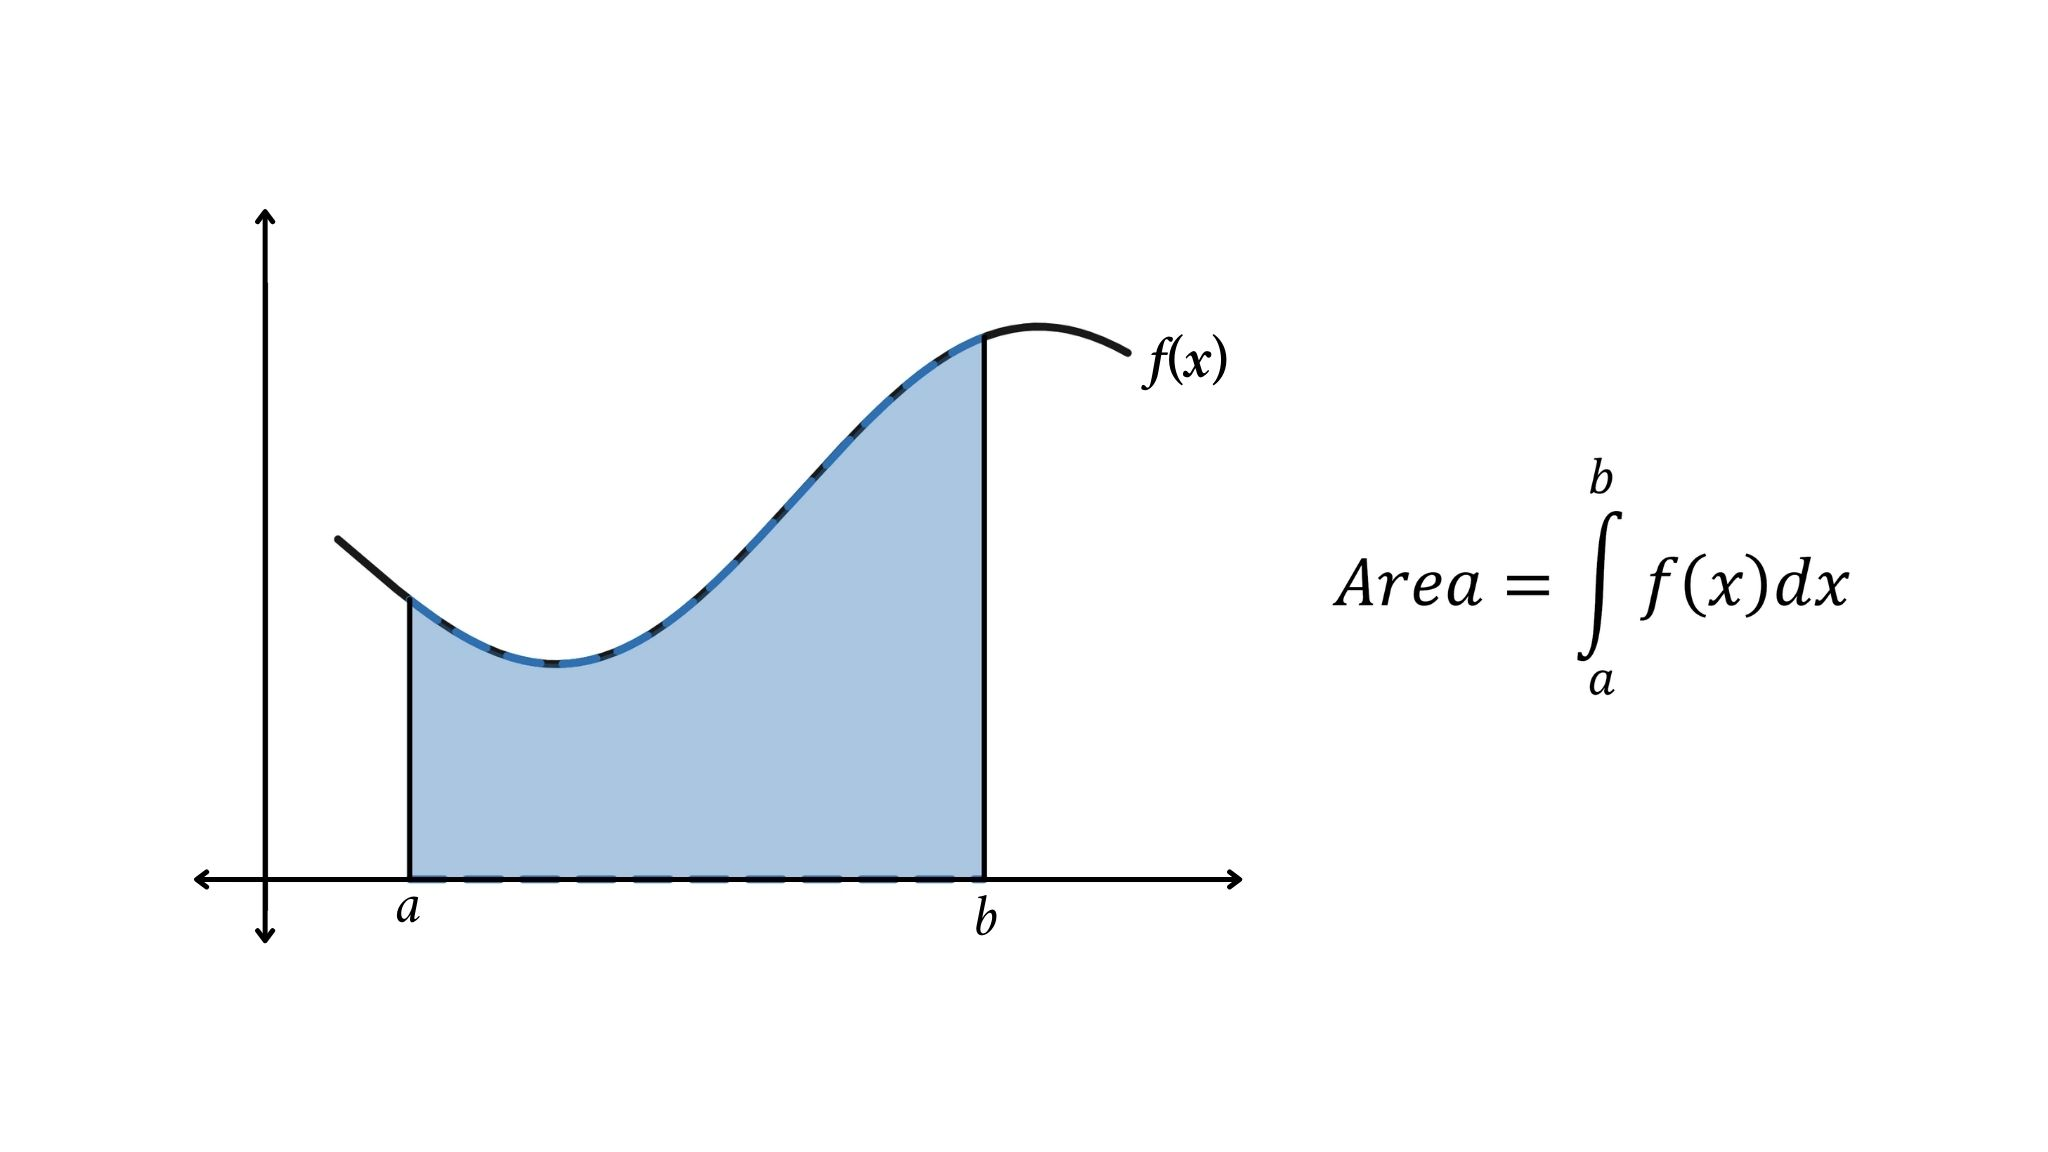
\includegraphics[width=0.8\linewidth]{figures/cover.jpeg}
    \caption{Area Under the Curve (AUC)}
\end{figure}

\begin{abstract}
    


In this report, we developed two complementary models for optimizing garbage truck dispersal across Manhattan districts MN1 to MN12. Our Deterministic model formulates the problem in terms of mixed integer programming. Systematically optimizing the time it takes for the trash collection.

Our Area Under the Curve (AUC) model, on the other hand, introduces a novel idea of measuring the environmental impact of leftover trash. It provides a more realistic approach by incorporating equity considerations, achieving a 68.92\% efficiency rate while maintaining fair service distribution across districts. 

By combining insights from both models, we demonstrate that a hybrid approach balancing deterministic scheduling with equity-based adjustments outperforms the current uniform distribution system. In addition, this model requires a significantly smaller proportion of trucks than available (maximum 64 trucks versus 2,230 available) while maintaining high service levels and equitable distribution across all districts.

%Our recommendation is a hybrid of the two system: times where there are high amounts of trash being produced in Manhattan, such as in and around holidays and during the summer, follow our schedule laid out by our deterministic model, and when normal amounts of trash are predicted to be produced.

\end{abstract}
\newpage

\tableofcontents

\newpage



\section{Introduction}

Having a system for picking up trash efficiently and respectfully is a crucial part of why Manhattan, and New York City as a whole, can remain the powerhouse it is today. However, having a uniformly spread-out schedule for all districts is not necessarily the layout of the garbage trucks in Manhattan to adhere to. In this report, we will prove this is the case.

We decided that the best course of action would be to divide the issue of garbage truck dispersal into a matter of efficiency and equity:

\begin{itemize}
    \item \textbf{Efficiency:} Each day, trucks need to be dispersed in a way such that they remove trash from all 12 districts as quickly as possible, leaving room to help other districts. This would ideally be with as little maintenance and fuel cost per truck as possible. However, our Deterministic model assumes ideal conditions without maintenance and fuel costs. Key metrics include:
    \begin{itemize}
        \item Total collection time per district
        \item Number of trucks required
        \item Utilization rate of each truck
        \item Time between pickups
    \end{itemize}
    
    \item \textbf{Equity:} We want our programs to be as fair as possible, with people in different regions receiving the same quality of service as much as possible. Although the definition of service quality varies, the notion of maintaining equity is consistent throughout our models.
\end{itemize}

% For robustness test, we will test the following:

% \begin{itemize}
%     \item \textbf{Disruptions:} This can have a variety of setbacks, such as failing to pick up trash, vehicle breakdowns, staff shortages, traffic delays, maintenance requirements, severe weather conditions, and events/holidays. For the purposes of our model, these are all co-factors of time, which in turn directly affects costs.
    
%     \item \textbf{System changes:} Variations in waste in a given season, and lowering the truck amount, are changes that significantly impact the efficiency and equity of waste collection across Manhattan.
% \end{itemize}

To address the problem of garbage collection comprehensively, it is essential to consider it from two distinct perspectives. On one side, sanitation workers aim to maximize collection efficiency, minimizing resource use—such as shift frequency and the number of trucks deployed. On the other side, residents want their household waste collected promptly, without it piling up in their homes or on the streets of Manhattan. To balance these needs, we developed two mathematical models that provide a structured approach to solving the problem.

These two models are fundamentally different in nature, the first one having the name of Deterministic model. The primary objective of this is to minimize the time it takes for sanitation workers to collect all the trash. Accounting for the time of trash pickup and vehicle commute. This model got its name from its deterministic nature, since it utilizes the optimization tool of mixed integer programming.

In contrast, our second model aims to quantify the social and environmental impact of delayed trash pickup. Its name reflects its approach, as it assesses the severity of trash buildup by integrating the amount of leftover trash over time. This is a novel and original idea inspired by concepts from other areas of natural sciences.
\newpage

\section{Model Assumptions}

\begin{itemize}
    \item \textbf{All trucks are the same:} While there are 275 specialized trucks within Manhattan’s fleet, these trucks only account for a small portion of all trucks available. to keep our models simple, we will consider these specialized trucks the same as normal trucks.

    \item \textbf{No traffic considerations:} Optimal conditions with no traffic delays, making pickup and route completion times predictable. Real-life conditions may vary significantly, particularly in districts with narrow streets or high pedestrian traffic.
    
    \item \textbf{Fixed pickup times (morning/evening slots):} Pickup times in the morning (7 AM - 8 AM) and evening (6 PM - 7 PM) are strictly adhered to, with no flexibility to shift times based on route completion or district demand.
    
    \item \textbf{Immediate pickup of trash:} Immediate pickup upon arrival at a location. All the pick-up speeds, if considered, are constant in any condition. This simplification excludes the possibility of delays due to operational factors like double-parking, parked vehicles obstructing access, or difficulties accessing bins, which can impact actual pickup times within districts. 
    
    \item \textbf{No stopping (continuous route completion):} Routes are completed continuously without additional, unplanned stops, simplifying route timing. In practice, trucks may need to stop for breaks, encounter unanticipated stops due to resident inquiries, or encounter other disruptions (e.g., loading delays).
        
    \item \textbf{Constant trash generation:} Each district generates a unique but constant amount of trash each day during the week. All trash that our models account for is generated in one of the 12 districts throughout the week.

    %\item \textbf{Each district can dispatch trucks: } For each of the 12 sanitation district, there is at least one garage available to dispatch trucks in the whole year.

    \item \textbf{Trash does not disappear:} Once trash is generated, it will not disappear unless it is collected.

    \item \textbf{Time discretization and truncation:} Since we do not have any hourly data on trash, we use days as our unit of time. For ease of calculation, scheduling and to account for the cyclical nature of the community, we have set the time span to one week.
\end{itemize}


\newpage

\section{Parameter values and their justifications}
In a problem that involves a lot of moving parts to maximize the efficiency and equity of when and where these trucks will go, we will break down the strongest contributors into simple parameters that can be easily interpretable for our models. 

\subsection{Parameter Table}

\begin{table}[h]
\begin{tabular}{|p{0.2\textwidth}|p{0.8\textwidth}|}
\hline
\textbf{Parameter} & \textbf{Description} \\
\hline
$\mathcal{D}$ & $\{1,2,\ldots,12\}$: District number, indexed by $d$ (e.g. MN1 to $d$=1)\\
\hline
$\mathcal{T}$ & $\{1,2,\ldots,7\}$: Days of the week from Sunday to Saturday, indexed by $t$ (e.g. Sunday to $t$=1)\\
\hline
$d$ & Dummy variable that always denote district ($d \in \mathcal{D}$) \\
\hline
$t$ & Dummy variable that always denote days ($t \in \mathcal{T}$)\\
\hline
$\mathcal{G}$ & Set of trucks \\
\hline
g & The label of individual truck\\
\hline
$C$ & Capacity of each truck in tons (e.g., 12 tons per truck) \\
\hline
$W_{d,t}$ & Daily waste generated in district $d$ on day $t$, in tons (randomly generated) \\
\hline
$h$ & Time taken to collect one ton of waste \\
\hline
$SEI_d$ & Socio-economic indicator for district $d$ \\
\hline
$f_d$ & Required pickup frequency in district $d$ (2--3 times per week) \\
\hline
$\alpha,\gamma,\beta$ & Weights for efficiency, equity, and maximizing garbage collection \\
\hline
$\mathcal{K}$ & $\{$Morning, Evening$\}$: Two available timeslots per day \\
\hline
$k$ & Index for timeslots (Morning = 7am--8am, Evening = 6pm--7pm) \\
\hline
$MaxTrucks$ & 2230: Maximum total number of trucks available across all districts and in deterministic model, it is set to be 500 trucks to reduce optimization complexity\\
\hline
$R_{d, t}$ & The number of tons of uncollected trash for district $d$ at day $t$ \\
\hline
$N_{d, t, s}$ & The number of trucks assigned to collect trash at district $d$ at day $t$ and time slot $s$\\
\hline
$P_{d}$ &  Population of district $d$\\
\hline
$AUC$ & The total $AUC$ of a schedule, for the definition of $AUC$, see \cref{sec:auc}\\
\hline
$AUC_d$ & The total $AUC$ of a district $d$\\
\hline
$AUC_{d,t}$ & The total $AUC$ of a district $d$, with respect to the time span $\{ 1, 2, ..., t \}$\\
\hline
\end{tabular}
\end{table}

\subsection{Parameter Justifications}

\begin{itemize}
    \item $\mathcal{T}$, $t$ and $\mathcal{K}$, $k$: The discretization of time into specific days ($\mathcal{T}$) and fixed timeslots ($\mathcal{K}$) reflects actual operational constraints of morning (7am--8am) and evening (6pm--7pm) collection windows, while simplifying the computational complexity of the model.
    \item $\mathcal{G}$: The total number of trucks available. To simplify our approach, we limit the fleet to approximately 500 trucks, as both models has the functionality of minimizing the number of trucks used.
    \item $C$, $h$: For model simplification, we assume uniform truck capacity ($C$=12 tons) and collection time per ton ($h$=1 minute/ton) across all vehicles, though these parameters typically vary based on truck specifications and operator efficiency in practice.
    \item $P_d$ and $SEI_d$: Similarly, we assume constant population ($P_d$) and socio-economic indicator ($SEI_d$) values for each district, though these metrics may fluctuate in reality.
    \item $W_{d,t}$ and $R_{d,t}$: These matrices track the waste generation ($W_{d,t}$) and remaining waste ($R_{d,t}$) for each district $d$ at time $t$, enabling efficient monitoring of waste accumulation patterns and facilitating comparative analysis.
    \item $N_{d,t,k}$: This three-dimensional matrix represents truck assignments to districts $d$ at time $t$ and timeslot $k$. Given our assumption of strict adherence to scheduled routes, this matrix allows us to directly influence the waste dynamics captured in $W_{d,t}$ and $R_{d,t}$.

    
\end{itemize}

\section{Model Formulation}

We have decided upon two different models to tackle this problem: the Deterministic model that focuses on complete weekly collection, and a Area Under the Curve (AUC) model that focuses on reducing environmental impact. While the Deterministic model prioritizes ensuring all trash is collected as quickly as possible, the AUC model considers both the timeliness of collection and the social impact of delayed collection across different districts. Our AUC model introduces the concept of Area Under the Curve of trash to quantify how long waste remains uncollected, allowing us to better address the varying needs and tolerances of different districts based on their population density and socioeconomic factors.

\begin{itemize}
    \item \textbf{Deterministic Model:} This model approaches the problem from an operational efficiency perspective, focusing on maximizing the amount of waste collected while minimizing resource usage. The primary goal is to optimize truck deployment and routing to collect as much trash as quickly as possible while adhering to the required 2-3 pickup frequency per district. This approach prioritizes predictable, scheduled pickups for each 12 district that streamlines operations and minimizes operational costs by maximizing the amount of trash picked up per minute. This model can further be divided into two different models, the fixed assignment model which limits each assigned truck in only one district and a truck sharing model which allows trucks to be shared across districts in different time slots in a week. 

    \item \textbf{AUC Model:} From the perspective of environmental and resident well-being, the longer uncollected garbage remains in a residential area, the more environmental problems and complaints it causes. The AUC model focuses on minimizing the time garbage remains uncollected after generation. By quantifying and optimizing these delays, the model creates a schedule that balances operational efficiency with community needs, while accounting for factors like fluctuating trash volume and district-specific requirements.
\end{itemize}

\subsection{Deterministic Model}

In order to gain insight on whether sharing trucks among districts reduces the total trucks used, the Deterministic Model is divided into two parts. The fixed assignment model and the shared model. We aim to optimize the distribution of trucks and the weekly pick-up frequency across all 12 districts. Our objective is to minimize the total collection time, maximizing the amount of garbage collected (efficiency), while ensuring that the proportion of garbage collected in each district remains consistent with the total amount generated (equity). This model uses mixed integer linear programming for optimization.

\subsubsection{Fixed Assignment Model}

\textbf{Randomly Generated Data Parameters}
\begin{itemize}
    \item \( \text{waste\_generated}_{d, \text{t}} \): Amount of waste generated in district \( d \) on day \( \text{t} \), drawn from a uniform distribution specific to each district with expectations equal to the realistic tonnage data
    \item \( \text{frequency\_required}_d \): Minimum required collection frequency for district \( d \).
\end{itemize}


\textbf{Decision Variables}
\begin{itemize}
    \item \( x_{d,g,k,\text{t}} \): Binary variable, 1 if truck \( g \) is assigned to district \( d \) during timeslot \( k \) on day \( \text{t} \), 0 otherwise.
    \item \( g_{d, \text{t}} \): Amount of garbage collected in district \( d \) on day \( \text{t} \) (continuous).
    \item \( \text{schedule\_used}_{d, \text{t}, k} \): Binary variable indicating if any truck is assigned to district \( d \) during timeslot \( k \) on day \( \text{t} \).
    \item \( z_{t,d} \): Binary variable, 1 if truck \( t \) is assigned to district \( d \) for any timeslot.
\end{itemize}


\textbf{Objective Function}
The objective is to minimize the following composite cost:
\[
\alpha \cdot TCT - \beta \cdot TGC + \gamma \cdot PGC
\]
where:

\begin{itemize}
    \item \( TCT \) (Total Collection Time) is given by:
    \[
    TCT = \sum_{d \in D} \sum_{g=1}^{\mathcal{G}} \sum_{k \in \text{Timeslots}} \sum_{\text{t} \in \text{Days}} x_{d,g,k,\text{t}} \cdot tct \cdot C
    \]
    \item \( TGC \) (Total Garbage Collected) is given by:
    \[
    TGC = \sum_{d \in D} \sum_{\text{t} \in \text{Days}} g_{d, \text{t}}
    \]
    \item \( PGC \) (Proportional Garbage Collection) is defined as the average absolute deviation from the mean of garbage collection proportions.
\end{itemize}


\textbf{Constraints}

\textbf{Garbage Collection Requirement:} Ensure the amount collected matches the truck capacity assigned.
\[
g_{d, \text{t}} = \sum_{g=1}^{\mathcal{G}} \sum_{k \in \text{Timeslots}} x_{d,g,k,\text{t}} \cdot C
\]

\textbf{Frequency Requirement:} Ensure each district has trucks operating a minimum and maximum number of times.
\[
2 \leq \sum_{g=1}^{\mathcal{G}} \sum_{k \in \text{Timeslots}} \sum_{\text{t} \in \text{Days}} x_{d,t,k,\text{t}} \leq 3
\]

\textbf{Scheduling Indicator Constraints:}
\begin{itemize}
    \item Upper bound:
    \[
    \text{schedule\_used}_{d, \text{t}, k} \leq \sum_{g=1}^{\mathcal{G}} x_{d,g,k,\text{t}}
    \]
    \item Lower bound:
    \[
    \sum_{g=1}^{\mathcal{G}} x_{d,g,k,\text{t}} \leq \text{schedule\_used}_{d, \text{t}, k} \cdot \mathcal{G}
    \]
\end{itemize}

\textbf{Distinct Schedule Requirement:} Limit the number of times schedules can be assigned to each district.
\[
2 \leq \sum_{\text{t} \in \text{Days}} \sum_{k \in \text{Timeslots}} \text{schedule\_used}_{d, \text{t}, k} \leq 3
\]

\textbf{Truck Assignment Constraint:} Ensure that each truck is assigned to exactly one district across all timeslots and days.
\[
\sum_{d \in D} z_{g,d} = 1, \quad \forall g \in \{1, \dots, \mathcal{G}\}
\]

\textbf{Truck-District Linkage:} Link \( x_{d,g,k,\text{t}} \) with \( z_{g,d} \) such that if \( z_{g,d} = 1 \), then truck \( g\) can be assigned to district \( d \).
\[
\sum_{\text{t} \in \text{Days}} \sum_{k \in \text{Timeslots}} x_{d,g,k,\text{t}} \leq z_{g,d} \cdot |\text{Days}| \cdot |\text{Timeslots}|
\]

\textbf{{Fixed Model Assessment}}

For the fixed model, the efficiency and equity of garbage collection across the 12 districts are assessed and optimized by balancing the Total Collection Time (TCT), Total Garbage Collected (TGC), and Proportional Garbage Collection (PGC). Here’s a breakdown of how these are modeled and the interpretation of the trade-offs between efficiency and equity:

\textbf{{Efficiency Assessment}}
In this model, efficiency refers to the Total Collection Time (TCT), which aims to minimize the amount of time trucks spend collecting garbage across districts. Efficiency is incorporated into the objective function as follows:

\[
\text{TCT} = \sum_{d \in \text{districts}} \sum_{t=1}^{\text{total\_trucks}} \sum_{k \in \text{timeslots}} \sum_{\text{day} \in \text{days}} x_{d,t,k,\text{day}} \cdot \text{truck\_collection\_time\_per\_ton} \cdot \text{truck\_capacity}
\]

The TCT component encourages minimizing the time trucks spend in each district, aiming for a lower operational time. Reducing TCT improves resource use and allows more collections within the same fleet capacity. Efficiency here, therefore, means achieving the garbage collection target while minimizing collection time and resources.

\textbf{{Equity Assessment}}
Equity in this model relates to the evenness of garbage collection among districts. It is measured by the Proportional Garbage Collection (PGC), which reflects the deviations in garbage collection proportions across the districts. Equity is assessed by calculating the deviations from a mean collection proportion:

\textbf{{Calculate Proportion for Each District:} }
The model first calculates the garbage collected/generated ratio (i.e., collected waste as a proportion of generated waste) for each district:

\[
\text{proportion}_d = \frac{\sum_{\text{day}} g_{d,\text{day}}}{\sum_{\text{day}} \text{waste\_generated}_{d,\text{day}}}
\]

\textbf{{Mean Proportion and Deviations:} }
The model then calculates the mean of these proportions across districts and introduces auxiliary variables to represent the positive and negative deviations from this mean.

\textbf{{Minimize Deviations:} }
The objective function includes the mean absolute deviation from this proportion, thus aiming to make garbage collection more equitable by keeping the proportions close to the mean.

\[
\text{PGC} = \frac{\sum \text{abs\_deviations}}{\text{len(proportions)}}
\]

\textbf{{Interpretation of Trade-offs}}

{Efficiency (TCT) vs. Equity (PGC):}
A higher weight on TCT ($\alpha$) encourages minimizing the time and resources used in garbage collection. This may prioritize larger or more accessible districts where collection is quicker and cheaper, potentially leading to an inequitable distribution where some districts are underserved. Conversely, a higher weight on PGC ($\gamma$) will encourage the model to focus on serving all districts equally, aiming to minimize deviations in the collection-to-generation ratios across districts. This may require extra time and resources to serve less accessible districts, potentially raising the TCT.

\textbf{{Efficiency vs. Maximizing Total Collection (TGC):}}
Emphasizing TGC ($\beta$) ensures that the total amount of garbage collected is maximized, which may lead the model to prioritize high-waste districts. This could indirectly improve efficiency by concentrating collection efforts where waste generation is highest, but it could lead to inequities if other districts are relatively neglected.

\textbf{{Equity vs. Total Collection (PGC vs. TGC):}}
If a high emphasis is placed on equity (PGC), the model might collect less total garbage (TGC) since it will be allocating resources more evenly rather than concentrating them on high-waste districts. In contrast, emphasizing TGC could lead to fewer resources in low-waste districts, sacrificing equity for a higher total collection.

\textbf{{Practical Implications}}
By tuning the weights $\alpha$, $\beta$, and $\gamma$, decision-makers can adjust the model to align with specific operational goals:

\begin{itemize}
    \item If the priority is efficiency, we would increase $\alpha$ to minimize TCT.
    \item If equity is critical, we would increase $\gamma$ to reduce deviations across districts.
    \item If maximizing collection is key, we would increase $\beta$ to favor TGC.
\end{itemize}

Balancing these objectives enables creating an operational plan that aligns with the city’s specific values and constraints, whether prioritizing efficient resource use, equitable service, or maximizing garbage collection across districts.



\subsubsection{Truck Sharing Model}

\textbf{Decision Variables}
$
x_{d,t,k,\text{day}} \in \{0,1\} \quad \text{Binary decision variable that is 1 if truck }  t \text{ is assigned to district }$ $ d \text{ at timeslot } k 
\text{ on day } \text{day}, \text{ otherwise 0.}
$
\[
g_{d,\text{day}} \geq 0 \quad \text{Amount of garbage collected by district } d \text{ on day } \text{day.}
\]
\[
\text{schedule\_used}_{d,\text{day},k} \in \{0, 1\} \quad \text{Binary decision variable that is 1 if a schedule (day, timeslot) is used in district } d, \text{ otherwise 0.}
\]
\[
\text{abs\_deviations}_i \quad \text{Absolute deviation in the proportion of collected garbage in each district compared to the mean proportion.}
\]

\textbf{Objective Function}

The objective function minimizes the weighted sum of:
\[
\text{Objective} = \alpha \cdot \text{TCT} - \beta \cdot \text{TGC} + \gamma \cdot \text{PGC}
\]
Where:
\[
\text{TCT} = \sum_{d \in D} \sum_{t \in T} \sum_{k \in K} \sum_{\text{day} \in D} x_{d,t,k,\text{day}} \cdot t_{\text{per ton}} \cdot C
\]
\[
\text{TGC} = \sum_{d \in D} \sum_{\text{day} \in D} g_{d,\text{day}}
\]
\[
\text{PGC} = \frac{\sum_{i=1}^{|D|} \text{abs\_deviations}_i}{|D|}
\]

\textbf{Constraints}

\textbf{Garbage Collection for Each District:}
\[
g_{d,\text{day}} = \sum_{t \in T} \sum_{k \in K} x_{d,t,k,\text{day}} \cdot C \quad \forall d \in D, \forall \text{day} \in D
\]

\textbf{Total Garbage Collected:}
\[
g_{d,\text{day}} \geq 0 \quad \forall d \in D, \forall \text{day} \in D
\]

\textbf{Frequency Requirement (each district can have 2 or 3 collections per week):}
\[
2 \leq \sum_{t \in T} \sum_{k \in K} x_{d,t,k,\text{day}} \leq 3 \quad \forall d \in D, \forall \text{day} \in D
\]

\textbf{Schedule Assignment: If any truck is assigned to a district on a given day and timeslot, then the schedule for that district must be used:}
\[
\sum_{t \in T} x_{d,t,k,\text{day}} \leq \text{schedule\_used}_{d,\text{day},k} \cdot |T| \quad \forall d \in D, \forall \text{day} \in \mathcal{D}, \forall k \in K
\]

\textbf{Limit on Schedules (each district can only use between 2 and 3 distinct schedules):}
\[
2 \leq \sum_{\text{day} \in \mathcal{D}} \sum_{k \in K} \text{schedule\_used}_{d,\text{day},k} \leq 3 \quad \forall d \in D
\]

\textbf{Truck Frequency (each truck can only be assigned to one schedule on any given day):}
\[
\sum_{k \in K} \sum_{\text{day} \in D} x_{d,t,k,\text{day}} \in \{0, 1, 2, 3\} \quad \forall d \in D, \forall t \in T
\]

\textbf{Unique Time Slot Assignment for Trucks:}
\[
\sum_{d \in D} x_{d,t,k,\text{day}} \leq 1 \quad \forall t \in T, \forall \text{day} \in D, \forall k \in K
\]

\textbf{Truck Sharing Model Assessment}


The truck-sharing model utilizes the same parameters, decision variables, and objective functions as our primary model but relaxes certain constraints to allow trucks to be shared across all 12 districts over seven days. To ensure practical feasibility, each truck is restricted to a single district per time slot on any given day, as the 1-hour time window is too short for both travel and trash collection according to geological data.

We argue that allowing truck sharing significantly reduces the number of trucks required per district rather than increasing it. This approach maintains that the proportion of trash collected in each district should be less than or equal to one, acknowledging that complete trash removal isn’t necessary at each interval. The increased flexibility of truck sharing optimizes the model by reducing the overall truck count and enhancing trash collection efficiency. By relaxing the restriction of trucks to a single district, we enable each truck to serve multiple districts as needed, leading to a reduction in total truck numbers, as our results confirm.

\subsubsection{Fixed Assignment Deterministic Model and Truck Sharing Deterministic Model side-by-side Cross Validation}

\begin{table}[H]
\centering
\begin{tabular}{|c|c|c|c|}
\hline
$\mathbf{(\alpha, \beta,\gamma)}$ & $\mathbf{E_{ef}}$ & $\mathbf{Mean Proportion}$ & $\mathbf{Proportion Variance/equity factor}$ \\ \hline
$(1,1,1)$    &     732         &  0.0862    &  0.0048      \\ \hline
$(1,1,0)$     &  996         &  0.1445  &   0.0806  \\ \hline
$(0,0,1)$      &   756         &   0.0920  &  0.0045    \\ \hline
\end{tabular}
\caption{Performance of the truck sharing model}
\label{tab:Fixed Assignment Model}
\end{table}

\begin{figure}[H]
	\centering
	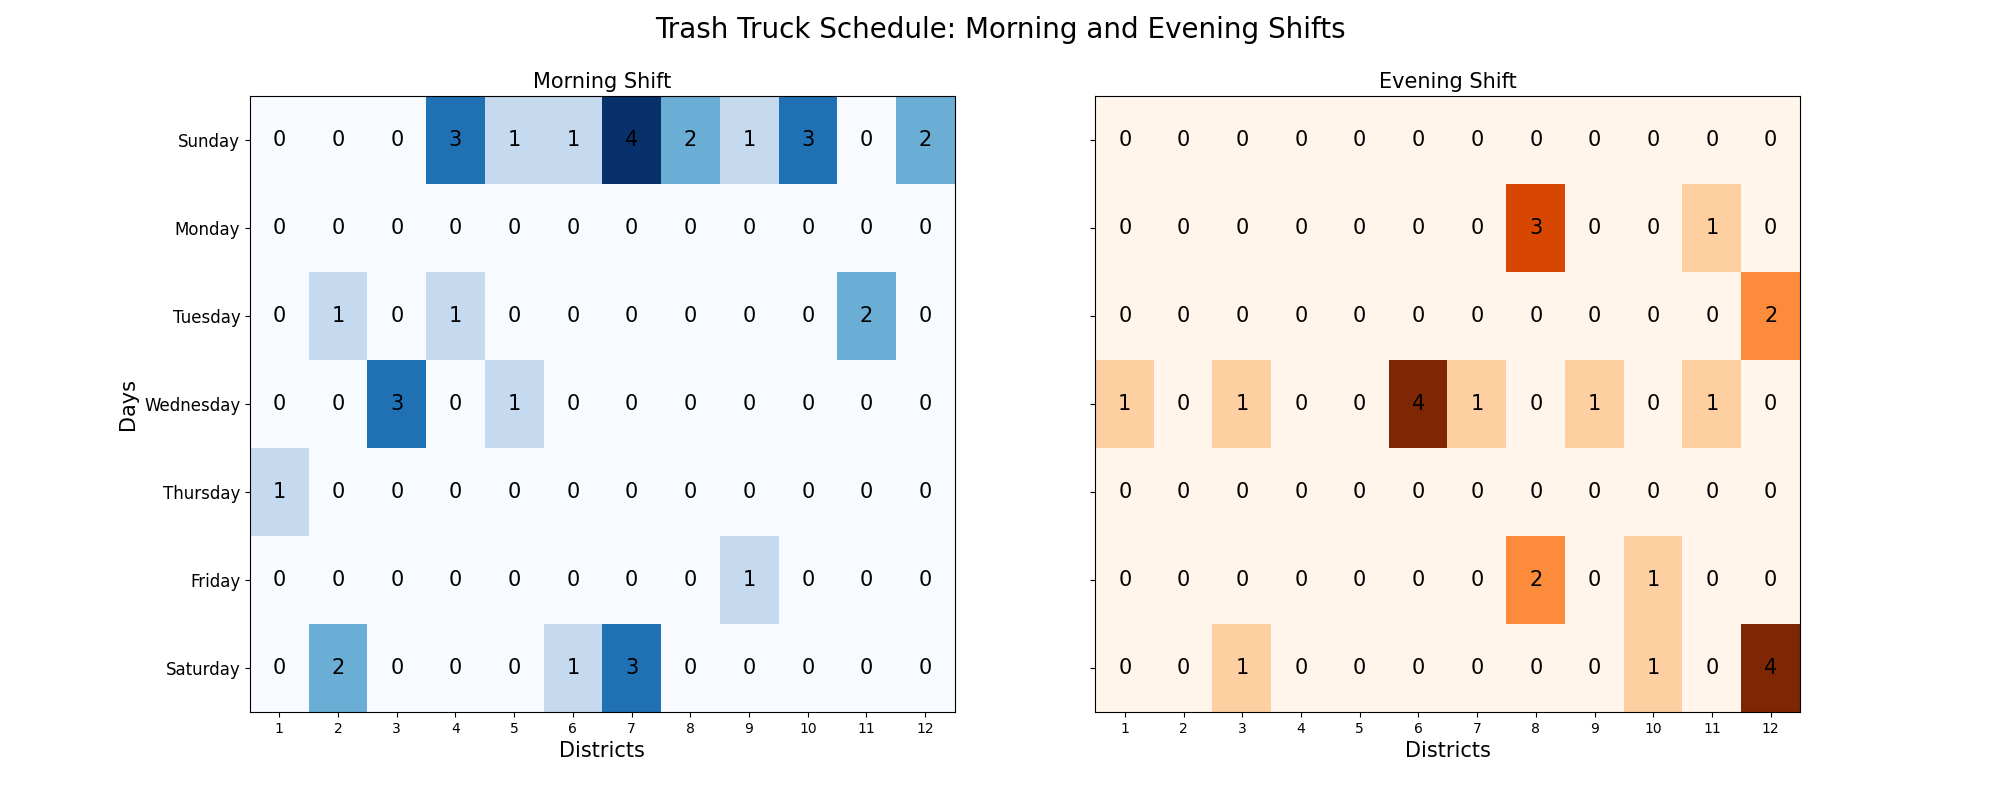
\includegraphics[width=1\textwidth]{figures/figures fixed/Prioritize TCT TGC PGC fixed model.png}
	\caption{Results for $(\alpha, \beta,\gamma) = (1,1,1)$. (variance =  0.0048, Mean\_proportion = 0.0862,$E_{ef} = 732$) In this case, the optimizer optimizes both efficiency and equity and it is the most balanced version in the three fixed models.}
	%\label{fig:1all}
\end{figure}

\begin{figure}[H]
	\centering
	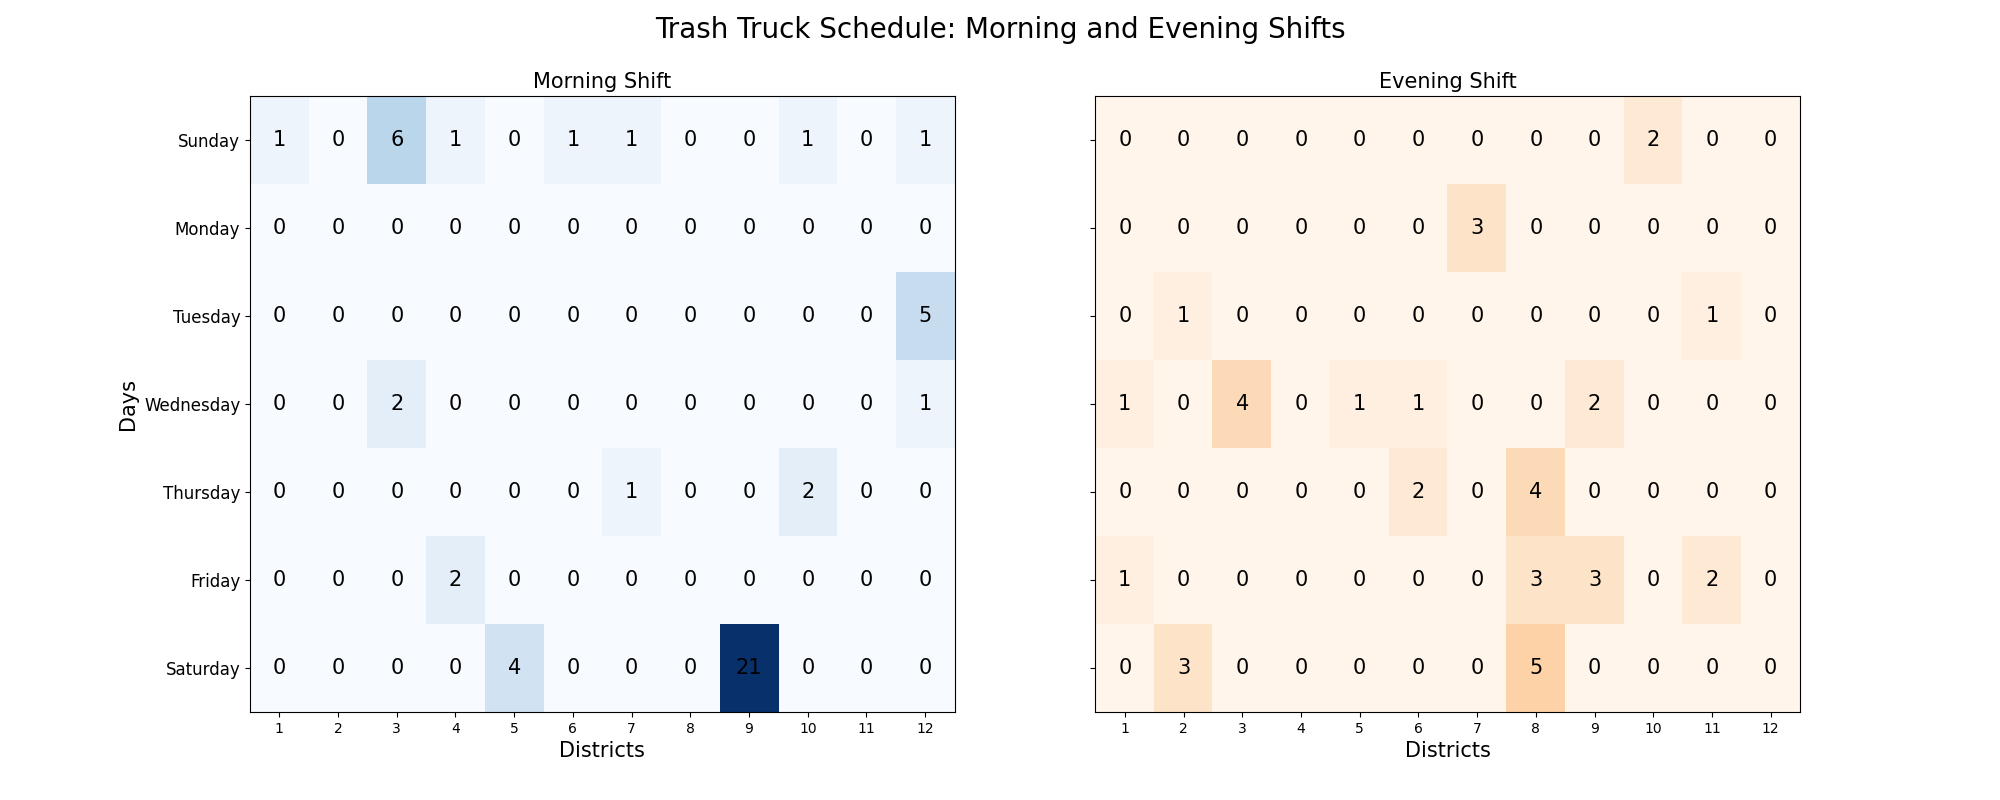
\includegraphics[width=1\textwidth]{figures/figures fixed/Prioritize TCT and TGC fixed model.png}
	\caption{Results for $(\alpha,\beta,\gamma) = (1,1,0)$. (variance = 0.0806(larger than 1,1,1), Mean\_proportion = 0.1445 , $E_{ef} = 996$) In this case, the optimizer optimizes only the efficiency and we can see the efficiency factor(the speed of garbage collection) is the largest while increasing the variance as the trade-off.}
	%\label{fig:1all}
\end{figure}

\begin{figure}[H]
	\centering
	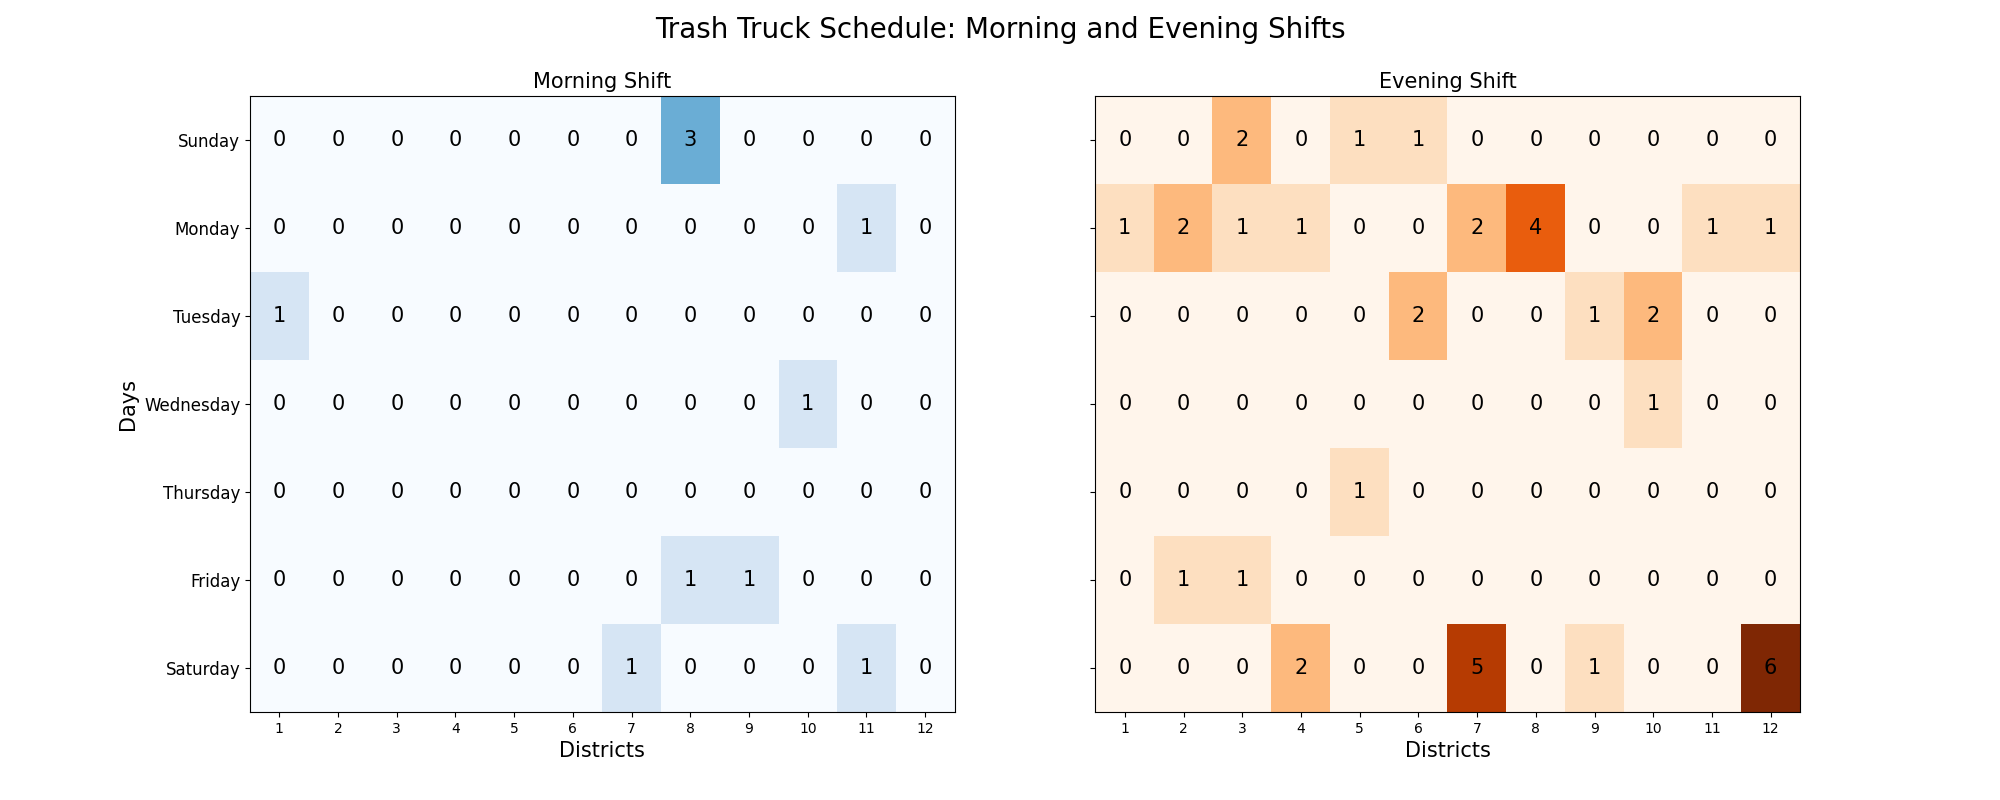
\includegraphics[width=1\textwidth]{figures/figures fixed/PGC fixed model.png}
	\caption{Results for $(\alpha, \beta,\gamma) = (0,0,1)$. (variance = 0.0045(best in equity), Mean\_proportion = 0.0920, $E_{ef}$$ = 756$) In this case, the optimizer optimizes only the equity and we can see the variance of mean proportions is the smallest among three fixed models. }
	%\label{fig:1all}
\end{figure}

\begin{table}[H]
\centering
\begin{tabular}{|c|c|c|c|}
\hline
$\mathbf{(\alpha, \beta,\gamma)}$ & $\mathbf{E_{ef}}$ & $\mathbf{Mean Proportion}$ & $\mathbf{Proportion Variance/equity factor}$ \\ \hline
$(1,1,1)$    &     1116         &  0.1450    &  0.0058      \\ \hline
$(1,1,0)$     &  10980        &  1.6845  &   0.5911  \\ \hline
$(0,0,1)$      &   864         &   0.1121  &  0.0046    \\ \hline
\end{tabular}
\caption{Performance of the truck sharing model}
\label{tab:TruckSharing}
\end{table}

\begin{figure}[H]
	\centering
	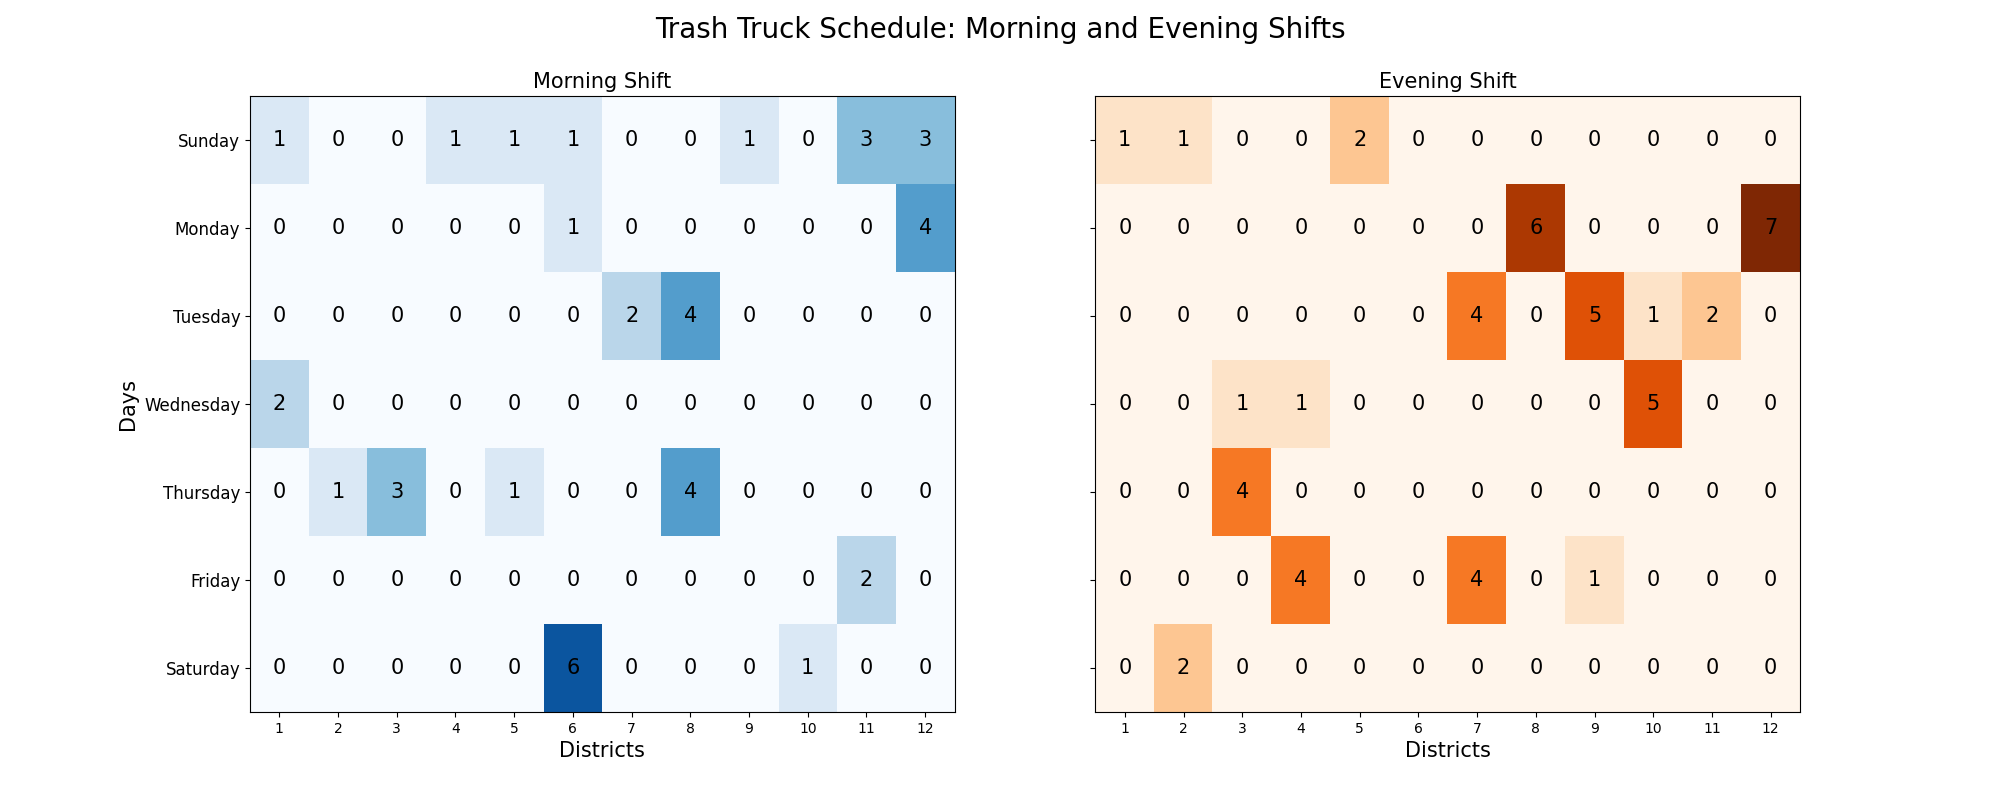
\includegraphics[width=1\textwidth]{figures/figures_shared/TGC TCT PGC sharing model.png}
	\caption{Results for $(\alpha, \beta,\gamma) = (1,1,1)$. (variance = 0.0058, Mean\_proportion = 0.1450,$E_{ef} = 1116$) In this truck sharing model, the optimizer optimizes both efficiency and equity and it is the most balanced version in the three truck sharing models.}
	%\label{fig:1all}
\end{figure}

\begin{figure}[H]
	\centering
	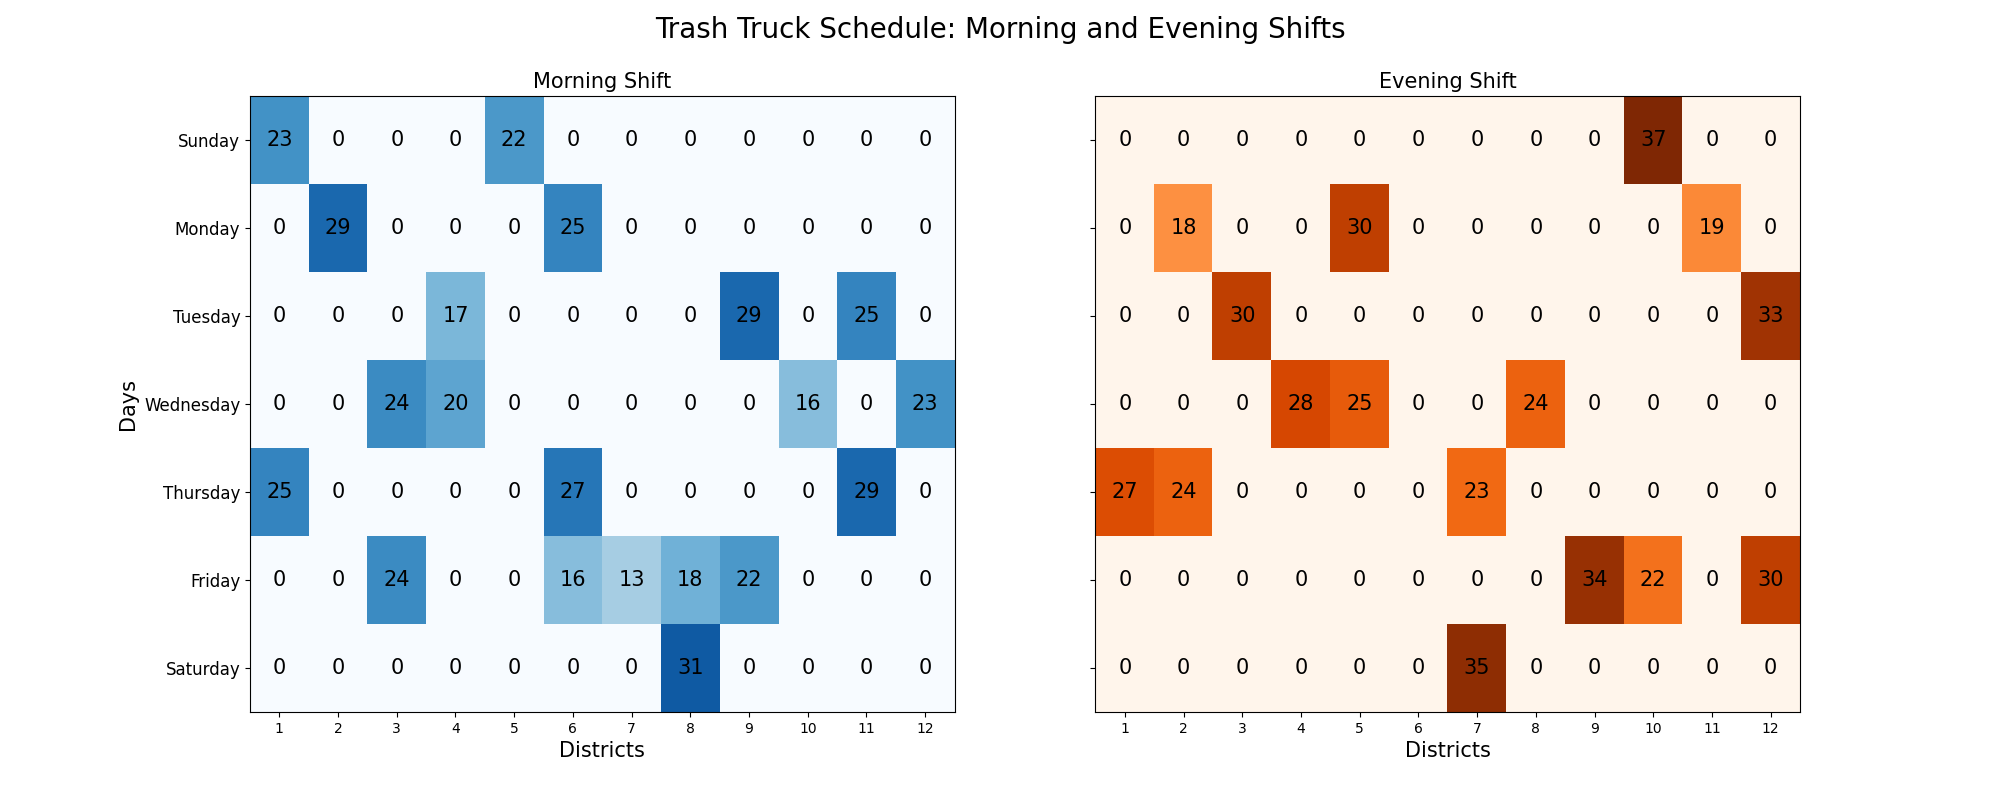
\includegraphics[width=1\textwidth]{figures/figures_shared/Prioritize TCT and TGC truck sharing.png}
	\caption{Results for $(\alpha,\beta,\gamma) = (1,1,0)$. (variance = 0.5911(much larger than 1,1,1), Mean\_proportion = 1.684456(the best among all the six models) , $E_{ef} = 10980$) In this case, the optimizer optimizes only the efficiency and we can see the efficiency factor(the speed of garbage collection) is the largest among all the six models while increasing the variance as the trade-off.And noticeably, the mean proportion is larger than 100\%, which means all the districts' trash could be cleaned up in this model's scheduling.}
	%\label{fig:1all}
\end{figure}

\begin{figure}[H]
	\centering
	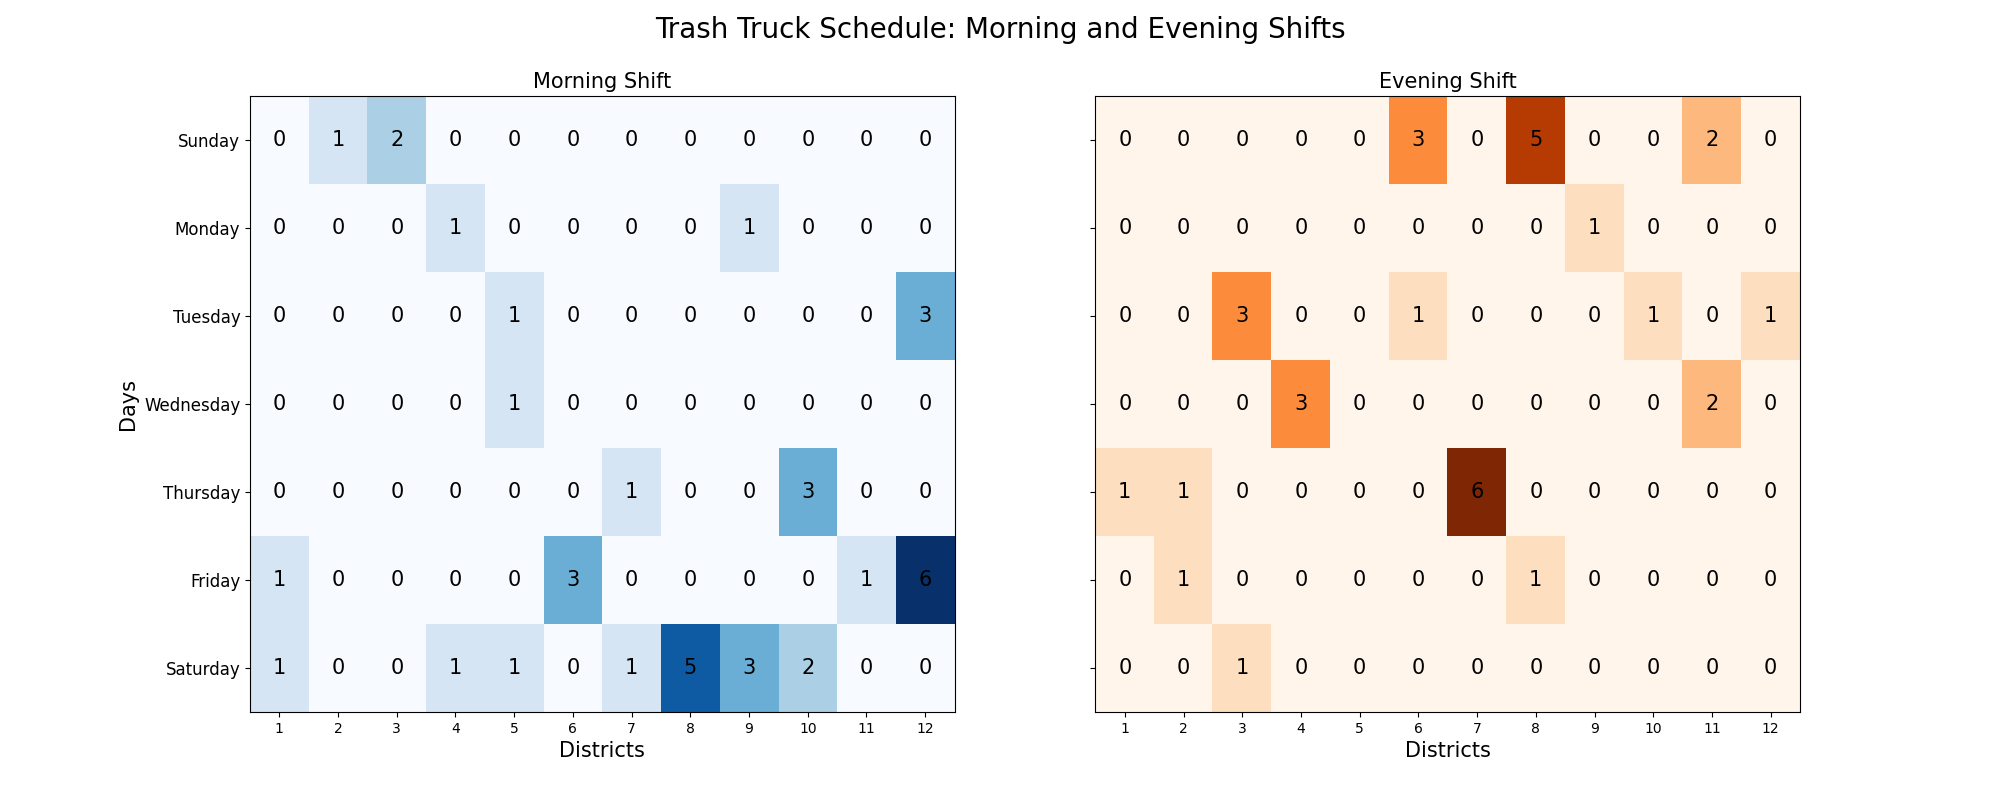
\includegraphics[width=1\textwidth]{figures/figures_shared/PGC sharing.jpg}
	\caption{Results for $(\alpha, \beta,\gamma) = (0,0,1)$. (variance = 0.0046, Mean\_proportion = 0.1121, $E_{ef}$$ =  864$) In this case, the optimizer optimizes only the equity and we can see the variance of mean proportions is the smallest among three truck sharing models, while the efficiency is the lowest in order to make the optimization feasible.}
	%\label{fig:1all}
\end{figure}


\subsection{AUC Model}

\subsubsection{Introduction to the AUC}
\label{sec:auc}

The term AUC (Area Under the Curve) is originally used in pharmacokinetics, where AUC is used to assess the total exposure of a drug or toxin in the bloodstream over time \cite{scheff2011assessment}, which is critical for determining appropriate dosages and understanding a drug’s efficacy and safety profile \cite{turner2020area}. 

Despite not being called AUC (but under the fancy name Riemann integral), the notion of integrating impact over time is far-reaching and deeply rooted in natural sciences. Physicists define Impulse as the AUC of force, deriving Newton's laws of motion, environmental scientists use AUC to calculate cumulative carbon emissions, informing climate change impacts, while engineers apply AUC to evaluate cumulative energy consumption, aiding in energy management and efficiency strategies.\footnote{Mathematicians manipulate AUC with set theory, inventing the even fancier Lebesgue integral}

In some sense, trash is to the city what toxins are to the human body. It is produced, transported, metabolized and eventually disappears with life activities. Thus, in analogy, if we happen to know the amount of uncollected trash $R(t)$ at a given time $t$, it is natural to quantify the impact of these uncollected trash in the time interval $[t_1, t_2]$ using the area under the curve:


\begin{align}
	AUC_d = \int_{t_1}^{t_2} R(t)_d dt \label{eq:AUC}
\end{align}

 If all trash are collected immediately once they are generated, then $ R_d(t) = 0$ for all $ t$ and $ AUC = 0$. While if do nothing in $[t_1, t_2)$ and suddenly collect all trash at once at time $ t_2$, then (if we assume there exists trash) $ AUC$ is positive. The end result of both processes is that all garbage is collected, but it is obvious that they have different environmental impacts, and $AUC$ portrays such differences.


From now on $AUC$ will be the variable by which we characterize the environmental and social impact of uncollected waste. Since in our problem the time was divided into 7 days, the weekly $ AUC$ for a district is calculated by:


\begin{align}
AUC_{d} = \sum_{t = 1}^{7} R_{d,t}	
\end{align}

Since we may also set the endpoint of our consideration to any day in the week, it is convenient to also define:

\begin{align}
    AUC_{d,t} = \sum_{j = 1}^{t} R_{d,j}
\end{align}

For any given day $t$.

\subsection{Determination of $W_{d,t}$}

Since we decided to simulate the creation and collection of garbage. $W_{d,t}$, the trash generated in district $d$ on day $t$ serves as a boundary condition for our calculation. Statistical data seems to provide useful information on this topic. See \cref{sec:hia} for more information. From historical data, we obtain $(m_d, \sigma_d)$, denoting the mean and standard deviation of daily trash generation for each district $d$ under suitable assumptions.

For simplicity, and due to the lack of additional data, we make certain realistic sacrifices to streamline our model, allowing us to assume:

\begin{align}
    W_{d,t} = m_d,  \forall d
\end{align}

On the other hand, $\sigma_d$ is used to test the robustness of our model under realistic fluctuations(see \cref{sec:senana}).

\subsection{Calculation of $R_{d,t}$}

\cref{alg:rcalc} Shows the procedure of calculating the uncollected trash $R_{d,t}$ with schedule $N_{d,t,s}$ and trash generation $W_{d,t}$. For every district $d$, at every day $t$, the uncollected trash from day $d - 1$ is passed to day $t$ (since we assumed that trash will not disappear unless it is collected). Next, the new trash generated $W_{d,t}$ is added to $R_{d,t}$. Finally, two collections according to $N_{d,t,s}$ is conducted. Leaving $R_{d,t}$ to be the uncollected trash for district $d$ on day $t$. Note that we do put an extra assumption that new trash is generated in the morning, we choose it to be in the morning so that the first day always has some trash to begin with.

\begin{algorithm}
\caption{Algorithm Calculating $R_{d,t}$ with $N_{d,t,s}$ and $W_{d,t}$}    \label{alg:rcalc}
\begin{algorithmic}
\State Set $R_{d,t} \leftarrow 0$
    \For{$d = 1$ \textbf{to} $12$} \Comment{Loop for districts}
        \For {$t = 1$ \textbf{to} $7$} \Comment{Loop for days}
        \If{$t > 1$}
        \State $R_{d,t} $+=$ R_{d, t - 1}$ \Comment{Uncollected trash from the previous day}
        \EndIf
        \State $R_{d,t} $+=$ W_{d,t}$ \Comment{New trash generated}
        \For {$s \in \mathcal{K}$}
        \State $R_{d,t} $ -=$ \min \{ R_{d,t}, C \cdot N_{d,t,s} \}$ \Comment{Subtract the trash collected}
        \EndFor
        \EndFor
    \EndFor
\end{algorithmic}
\end{algorithm}

\subsubsection{Efficiency}

The efficiency of a schedule is calculated by:

\begin{align}
    E_{ef} = \frac{\mbox{trash collected}}{C \cdot \mbox{trucks used}} \label{eq:eefdef}
\end{align}

This measures the extent to which the trash truck’s capacity is utilized.

Note that we may also define

\begin{align}
    \frac{AUC}{\mbox{trucks used}}
\end{align}



for efficiency, or simply use the number of trucks used(for optimization purposes). We decided that the definition in \cref{eq:eefdef} has more universality, meaning that it coincides more the the intuitive notion of efficiency in real life.

\subsubsection{Equity}

For each district $d$, we calculate a Equity factor $E^{eq}_d$ according to $AUC_d$ and it's population $P_d$ and socioeconomic factor $SEI_d$:

\begin{align}
    E^{eq}_d = \frac{AUC_d \cdot SEI_d}{P_d}
\end{align}

The Equity factor quantifies the impact of delayed waste collection on each district, averaged out with district population $P_d$ and socioeconomic factor $SEI_d$. Since fairness should be weighed \textbf{Per Capita}, thus the Equity factor of a district is inversely proportional to the population of that district. We multiply by a district specific socioeconomic factor to accommodate different circumstances, while this number is set to 1 in the AUC model.

The overall Equity factor $E_{eq}$ of a schedule is measured by taking the square root of the sample variance of $E_d^{eq}$ as $d$ varies:

\begin{align}
    E_{eq} = \sqrt{\mbox{Var}[E_d^{eq}]}
\end{align}

The larger the value of $E_{eq}$, the less equity a schedule has, since larger $E_{eq}$ would imply larger deviations of $E^{eq}_d$ among districts.

% ensuring our model prioritizes resource allocation to districts with higher population densities and consequently greater waste generation rates.

\subsubsection{Optimization function}

The overall loss function is defined by:

\begin{align}
    \mathcal{L} = \sum_{d \in \mathcal{D}} AUC_d - \lambda_1 \cdot E_{ef} + \lambda_2 \cdot E_{eq}
\end{align}

Minimizing $\mathcal{L}$ would minimize total $AUC$ and $E_{eq}$, while maximizing $E_{ef}$. By changing the values of $\lambda_1$ and $\lambda_2$, we can alter the relative importance of equity and efficiency.

Since there are non-linear terms in $E_{eq}$ and the acquisition of $AUC$ requires complicated manipulation of $W_{d,t} $ and $ N_{d,t,s}$, it is hard to came up with a systematic optimization method for this problem. Since $\mathcal{L}$ is only dependent on $N_{d,t,s}$ when $W_{d,t}$ is given, we use a stochastic method of randomly perturbing $N_{d,t,s}$ and in the process, minimize $\mathcal{L}$.

\section{Model Predictions}

\subsection{AUC Model results}

Result visualizations of the AUC model are shown in \cref{fig:1all}, \cref{fig:2all}, \cref{fig:3all}, \cref{fig:4all}, \cref{fig:5all}. Each summary consists of four vertical arranged graphs. Beginning with the visualization of the schedule, where darker color denotes more trucks assigned. The second graph shows $R_{d,t}$, the remaining uncollected trash each day. The third graph shows $AUC_{d,t}$, which is the integral of $R_{d,t}$ with respect to $t$. Note that for the following analysis, only $AUC_{d,t}$ when $t = 7$ (Saturday) is used for calculation, while the $AUC_{d,t}$ for the rest of the days are show for the sake of completeness. The fourth graph shows $AUC_{d,t}$ averaged by the population of each district, whose fluctuation among districts depicts equity.


The results are summarized in \cref{tab:AUCresults}.

\begin{table}[H]
\centering
\begin{tabular}{|c|c|c|c|}
\hline
$\mathbf{(\lambda_1, \lambda_2)}$ & $\mathbf{E_{ef}}$ & $\mathbf{E_{eq}}$ & $\mathbf{AUC}$ \\ \hline
$(0,0)$                  & 0.52     & 3.85     & 5520  \\ \hline
$(100,0)$                & 1.00     & 35.84    & 10940 \\ \hline
$(1,0)$                  & 0.71     & 4.91     & 5426  \\ \hline
$(0,1)$                  & 0.55     & 3.42     & 6226  \\ \hline
$(1,1)$                  & 0.69     & 2.53     & 5636  \\ \hline
\end{tabular}
\caption{Result summary of the AUC model}
\label{tab:AUCresults}
\end{table}

These results shows a complex scheduling pattern where districts require diverse collection times, including Saturday pickups beyond traditional working hours. Notably, several districts receive substantial service during evening shifts (e.g., District 8 with 52 trucks on Wednesday evening in \cref{fig:5all}), while others maintain consistent morning collections (e.g., District 1's pattern of morning pickups on Tuesday, Thursday, and Saturday in \cref{fig:5all}).

Since we used statistical data from reality to simulate trash generation. It is informative in a since that if we neglect uncertainties and maintain high efficiencies, it actually does not require many trucks to be effective and equal, with the most busy of days not exceeding 223 trucks. Thus of the 2,230 trucks in New York City, we have a manageable number of trucks that we can utilize.

One consistent anomaly in our model appears to be districts 7 and 8 having high amounts of trash left over, but this likely due to our model being limited to going 2-3 times a week per district and, district 7 and 8 being the most densely populated districts (209084 and 219920 in 2010 respectively).

Another anomaly in our model is that among all these choices of $(\lambda_1, \lambda_2)$, hardly ever does the optimizer assign trucks to work on Sunday. This accidentally coincides with the reality that DSNY doesn't work on Sundays (The optimizer does not know this fact. Or doesn't it?). We believe that the reason for this result is that the optimizer doesn't think that the garbage generated on the first day is worth consuming a garbage collection for. Since we are under the constraint of only collecting 3 times for each district.

That is not to say that our loss function is superior to other alternative metrics. One example is the amount of trash left at the end of the week. ($(\lambda_1, \lambda_2) = (0,0)$, \cref{fig:1all}) is pretty promising in terms of this. However, this is to be expected, as this model does not account for a reasonable limit to the amount of trucks needed, nor the need to accommodate for the equality of trash levels in each district.

In addition, $(1,0)$ and $(0,1)$, scenarios that accommodate for only efficiency or only equity resulted in exact levels of unoptimal amounts of remaining trash by the end of the week, as to be expected, since our loss function does not penalize for weekly trash remain.

Finally, our optimal model appears to be that of \cref{fig:5all}, which balances efficiency over equity (weighted by $\lambda_1$=1 and $\lambda_2$=1 respectively), minimizes the total residual waste across all districts by the end of the simulated week.

\begin{figure}[H]
	\centering
	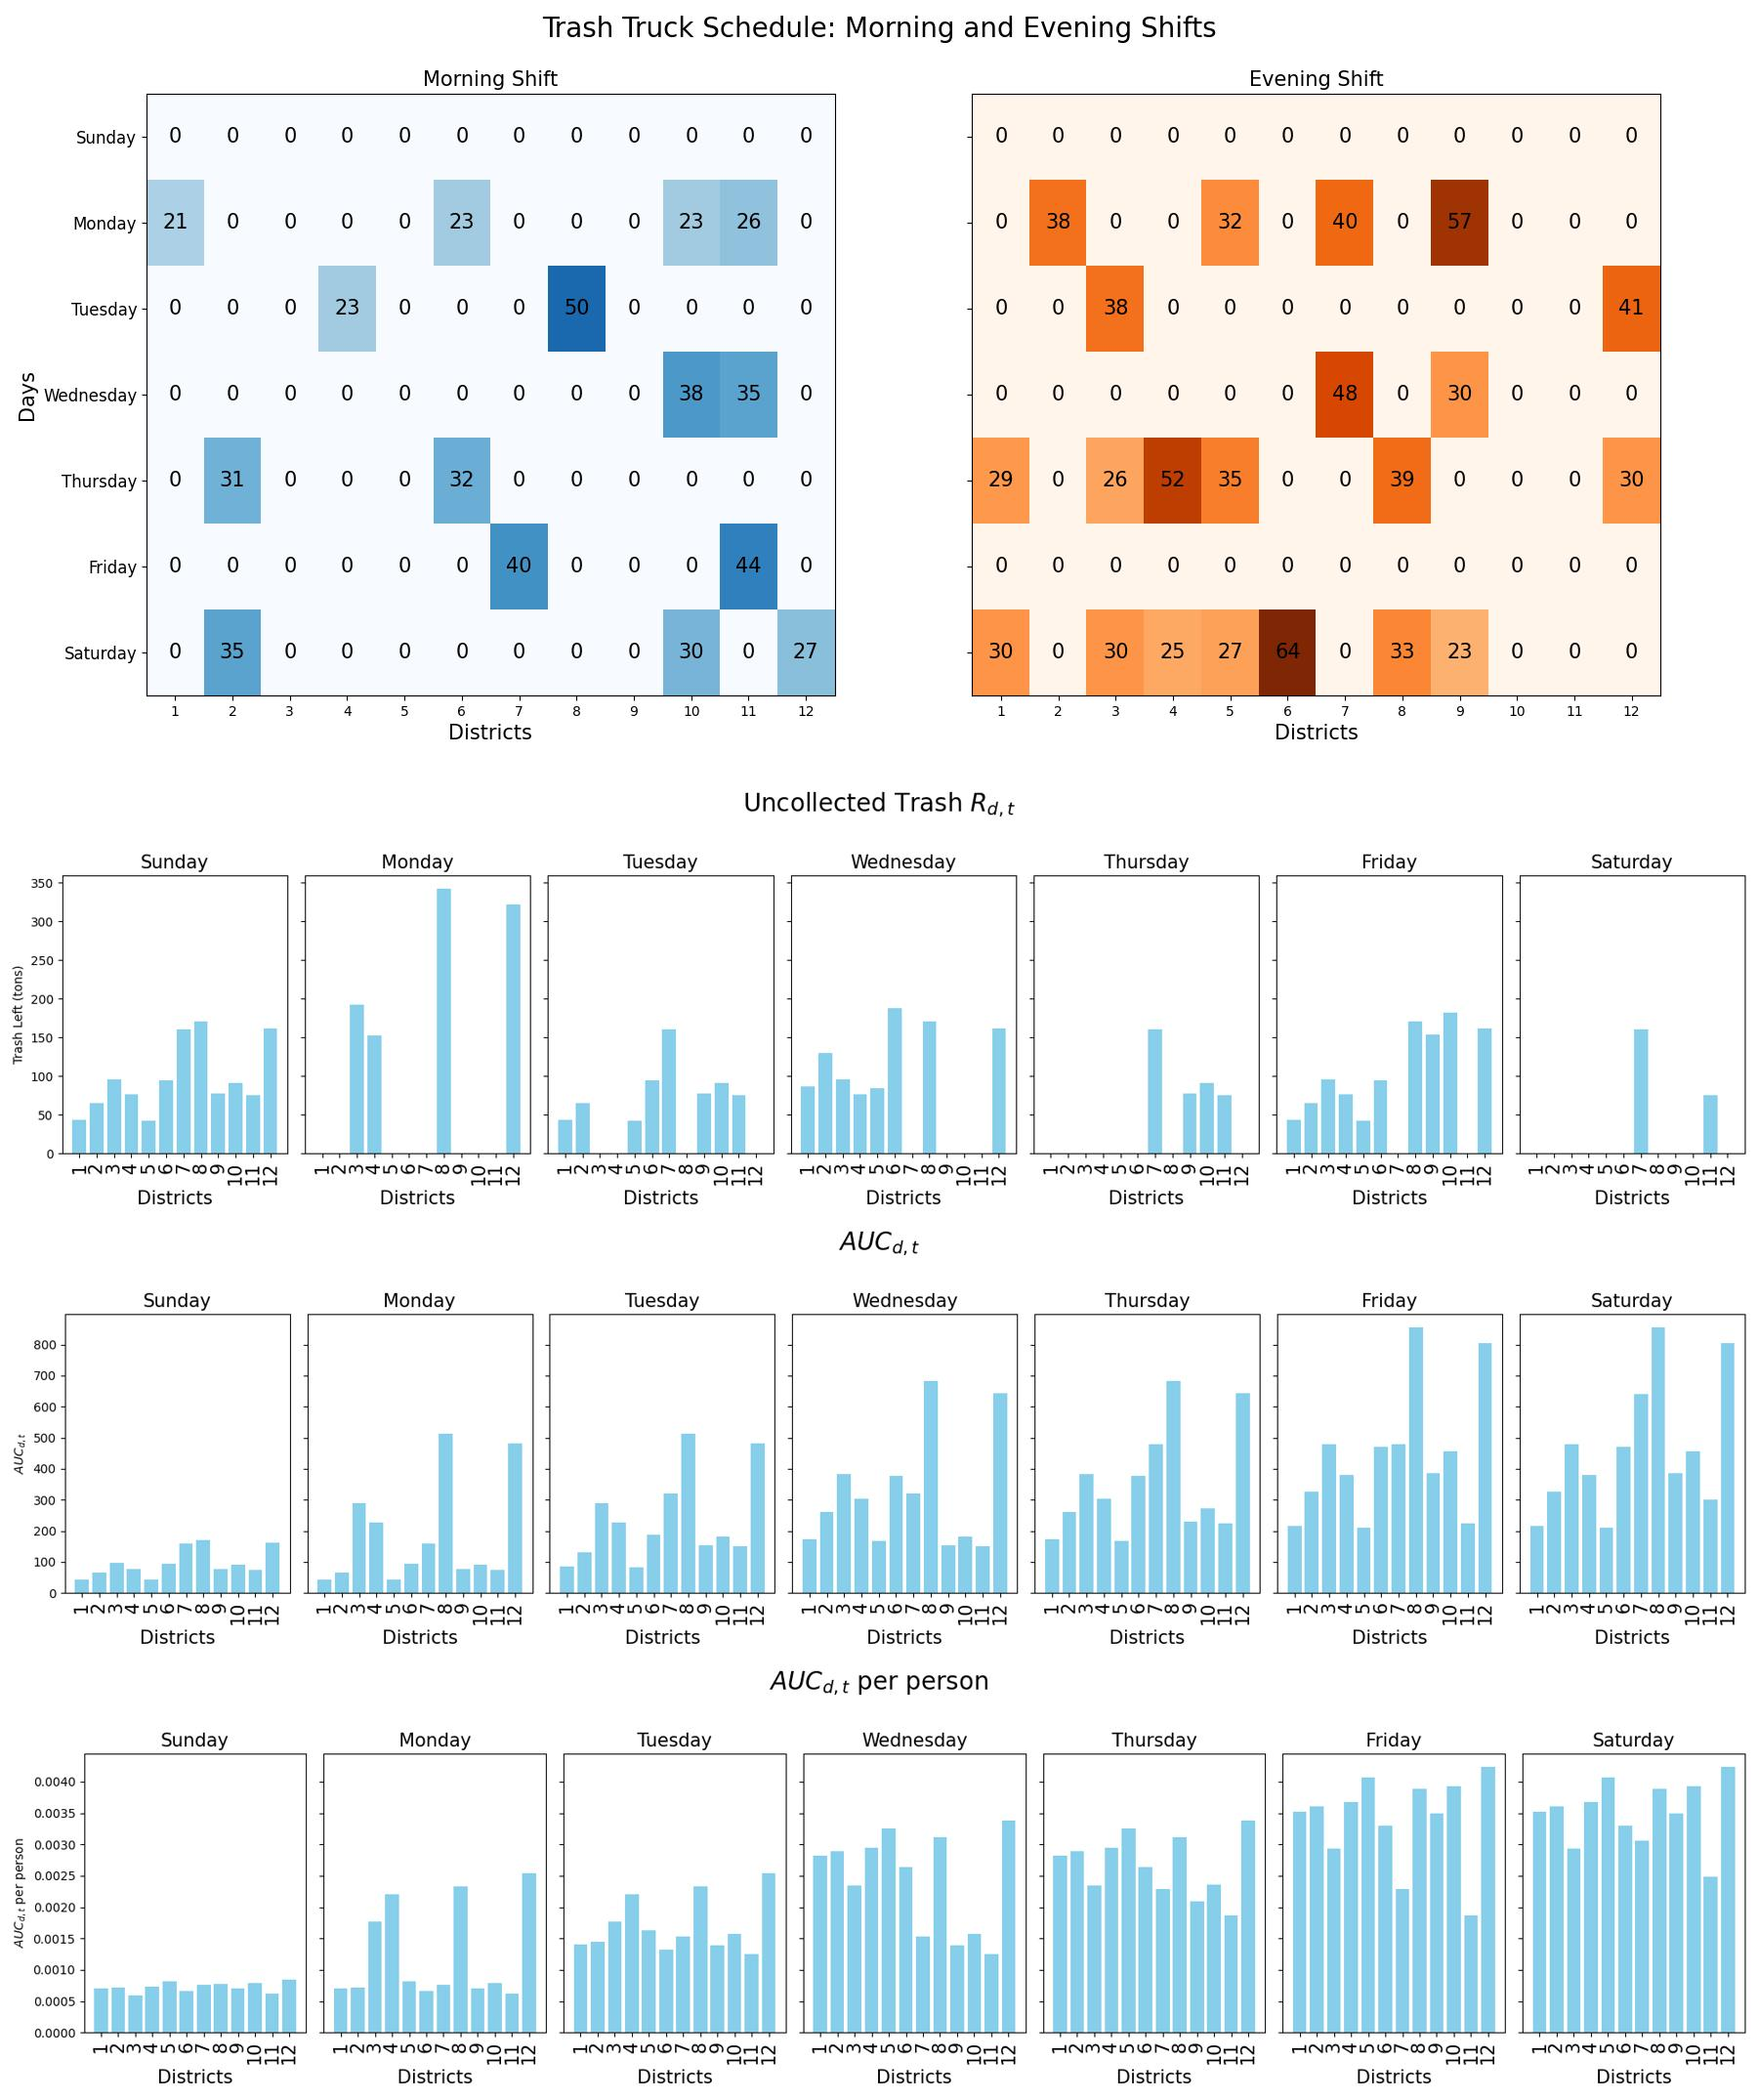
\includegraphics[width=1\textwidth]{figures/(0,0).jpg}
	\caption{Results for $(\lambda_1, \lambda_2) = (0,0)$. ($AUC = 5520.0, E_{eq} = 3.85, E_{ef} = 0.52$) In this case, the optimizer only optimizes total AUC, neglecting efficiency and equity, thus although most trash are collected at the end of the week, an excessive number of trucks are used, resulting in an overall efficiency of 52.36 \%. }
	\label{fig:1all}
\end{figure}

\begin{figure}[H]
	\centering
	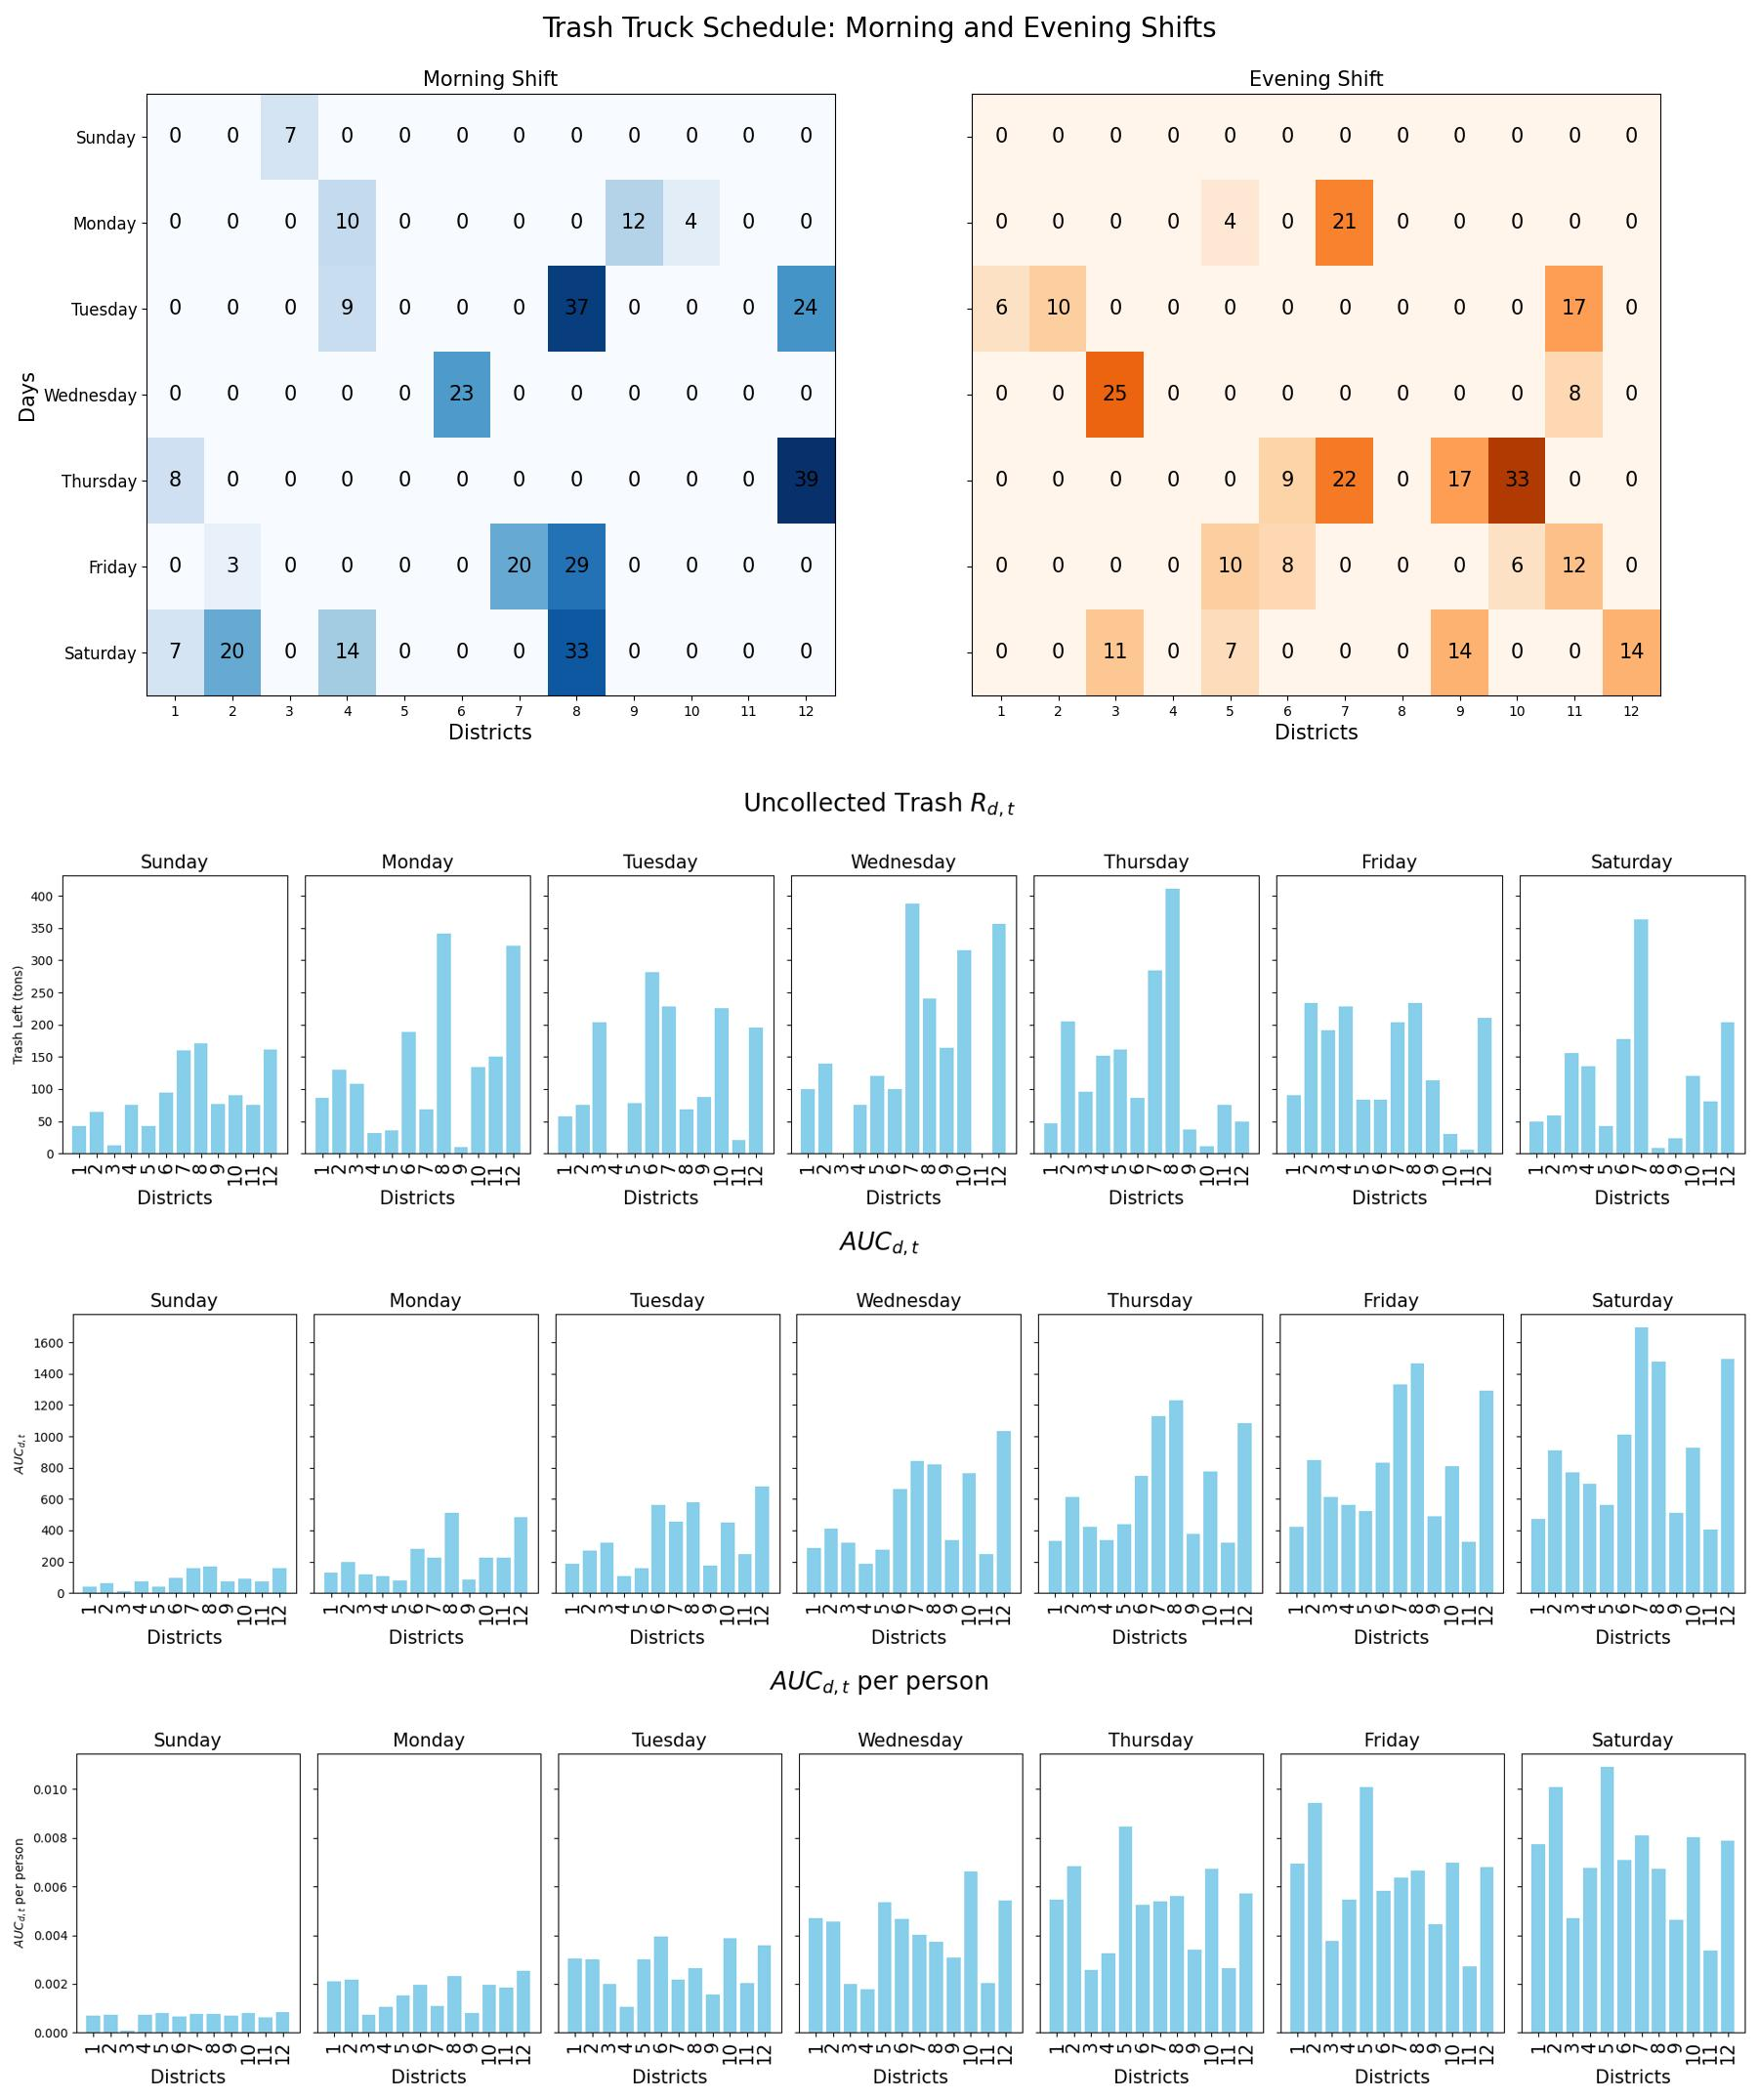
\includegraphics[width=1\textwidth]{figures/(100,0).jpg}
	\caption{Results for $(\lambda_1, \lambda_2) = (100,0)$. ($AUC = 109030.0, E_{eq} = 35.84, E_{ef} = 1.00$) In this case, the optimizer prioritizes efficiency to an extreme, reaching an overall efficiency of 100\%, however, a minimal amount of trucks are used and the overall $AUC$ is high. Since we neglected equity, $AUC$ per person varies a lot among different districts.}
	\label{fig:2all}
\end{figure}

\begin{figure}[H]
	\centering
	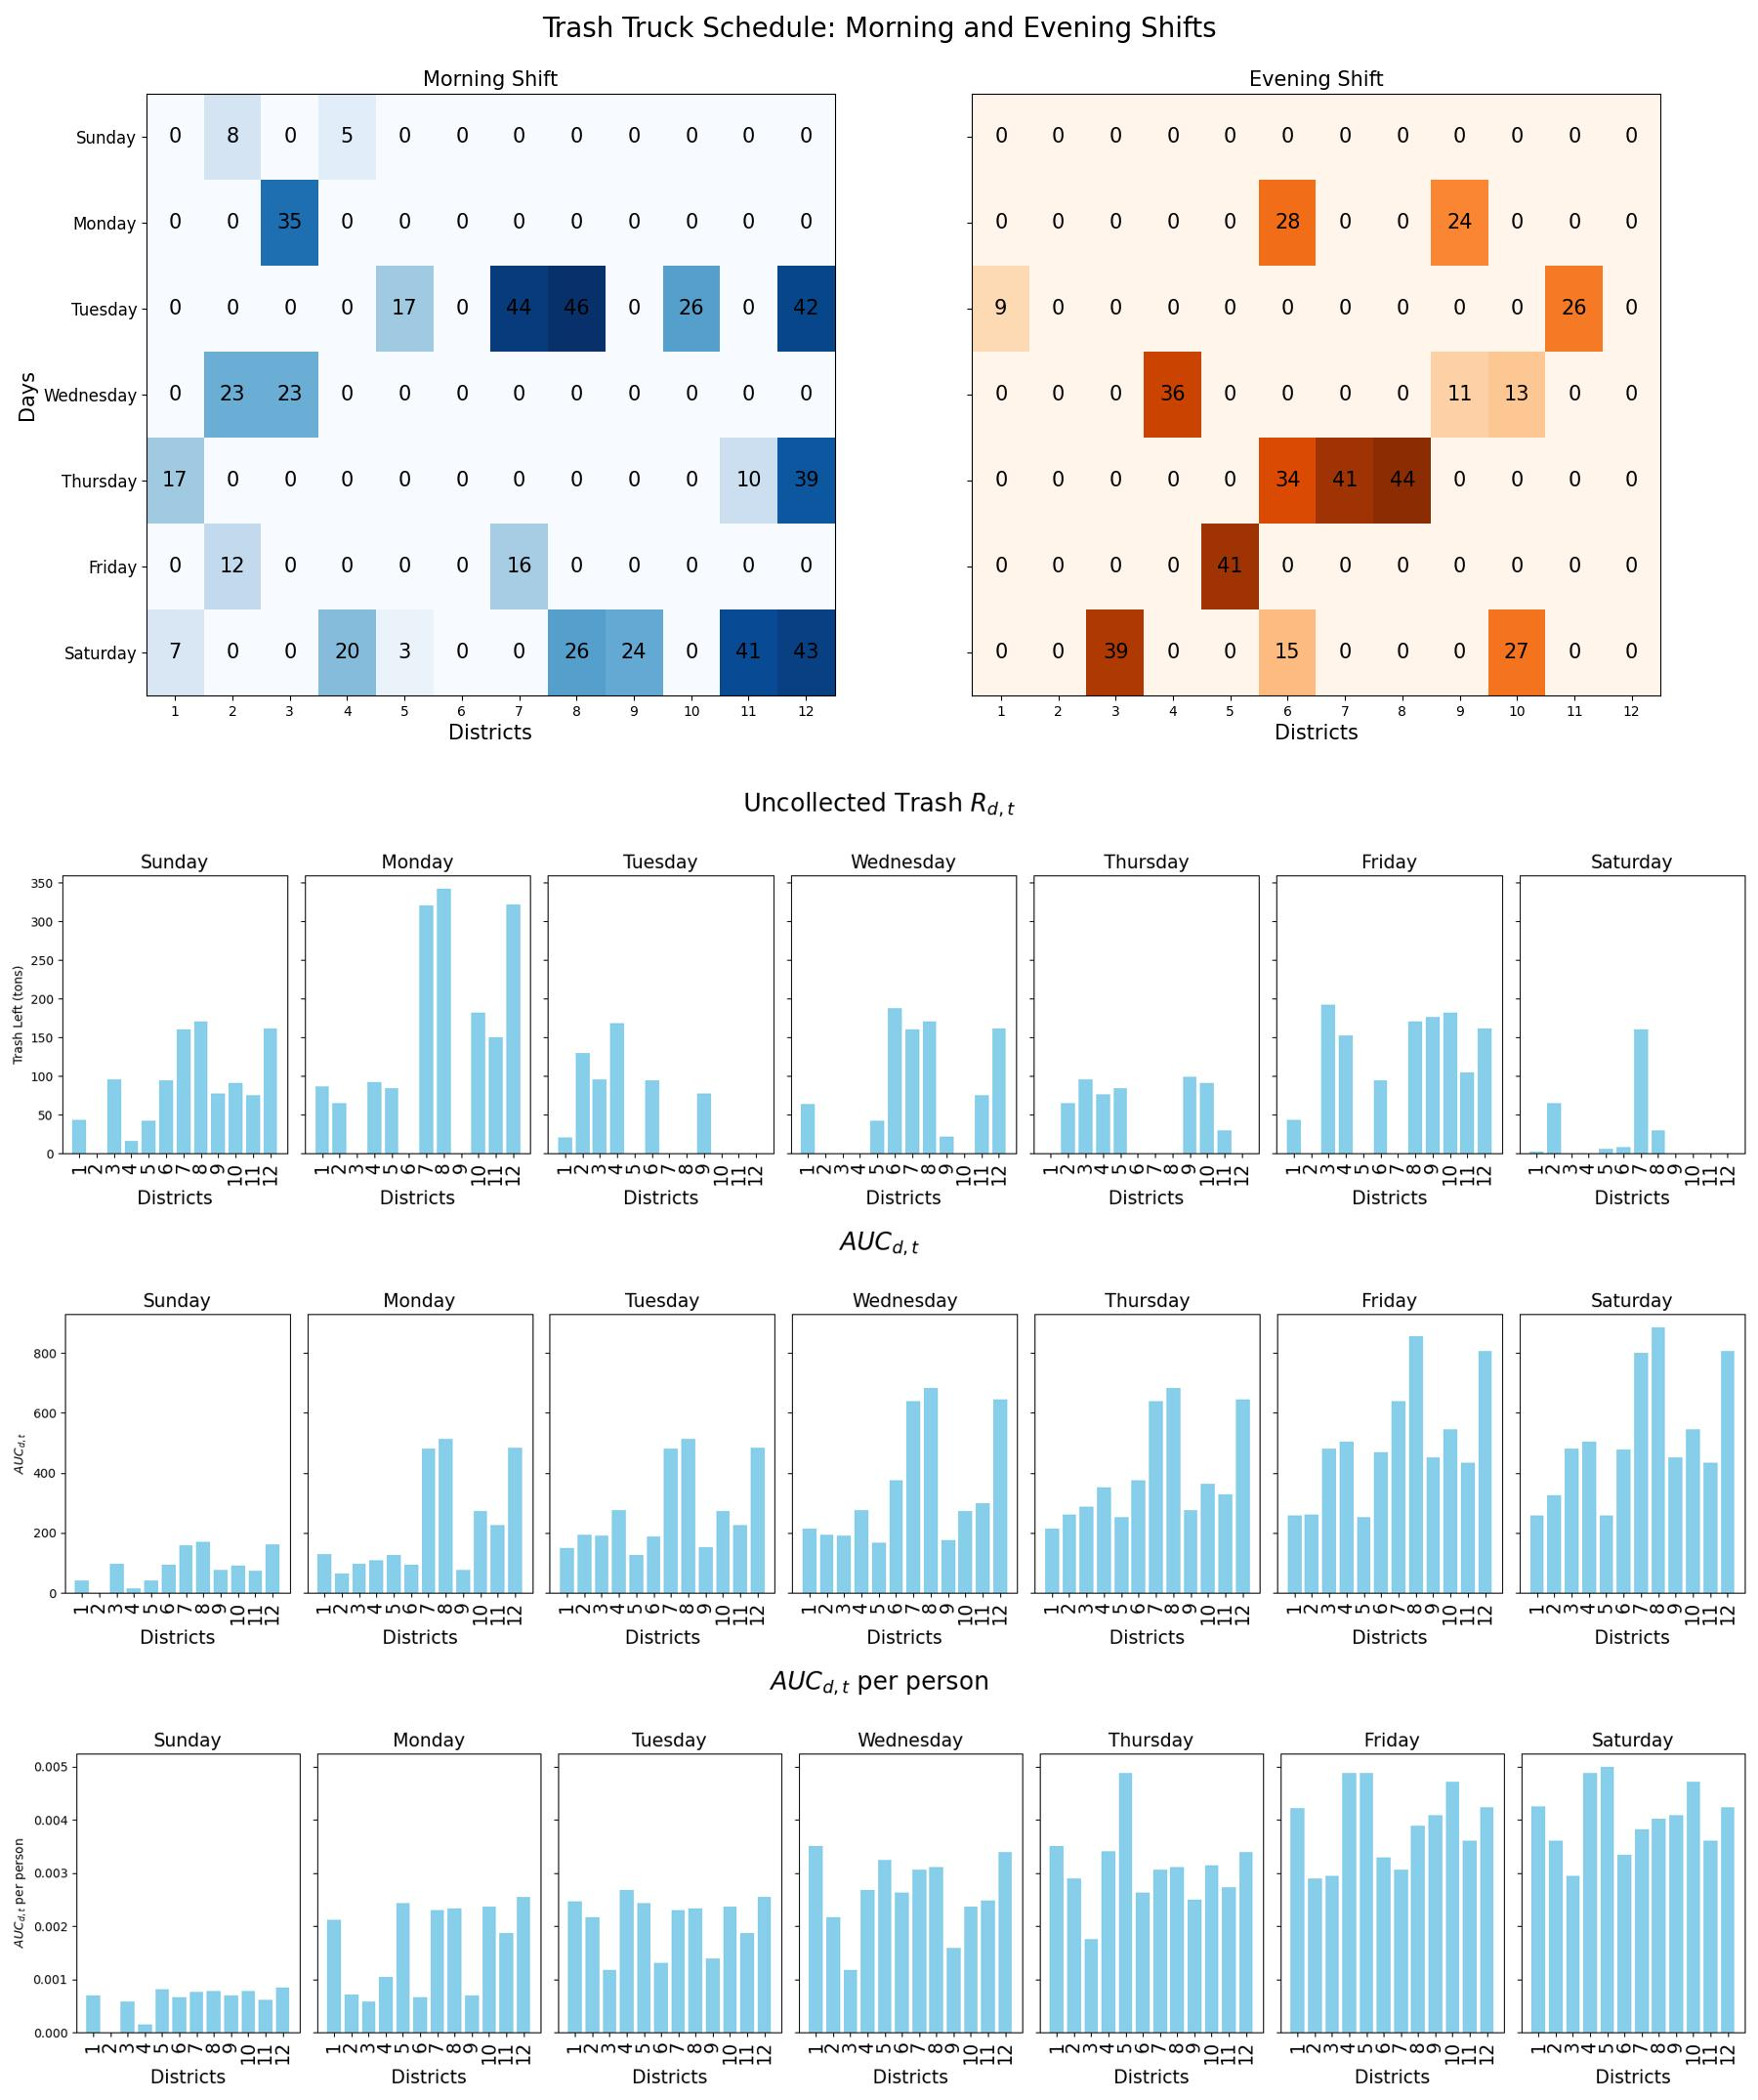
\includegraphics[width=1\textwidth]{figures/(1,0).jpg}
	\caption{Results for $(\lambda_1, \lambda_2) = (1,0)$. ($AUC = 6226.0, E_{eq} = 4.91, E_{ef} = 0.71$) In this case, the optimizer prioritizes efficiency, but not to an extreme, which results in an overall efficiency of 70.91\%. The variance of AUC per person is lower than the case of $(100,0)$. Although we did not take equity into account in terms of the loss function, a comparison with $(\lambda_1, \lambda_2) = (100,0)$ (\cref{fig:2all}) does indicate that one might lose equity in the pursuit of efficiency. }
	\label{fig:3all}
\end{figure}

\begin{figure}[H]
	\centering
	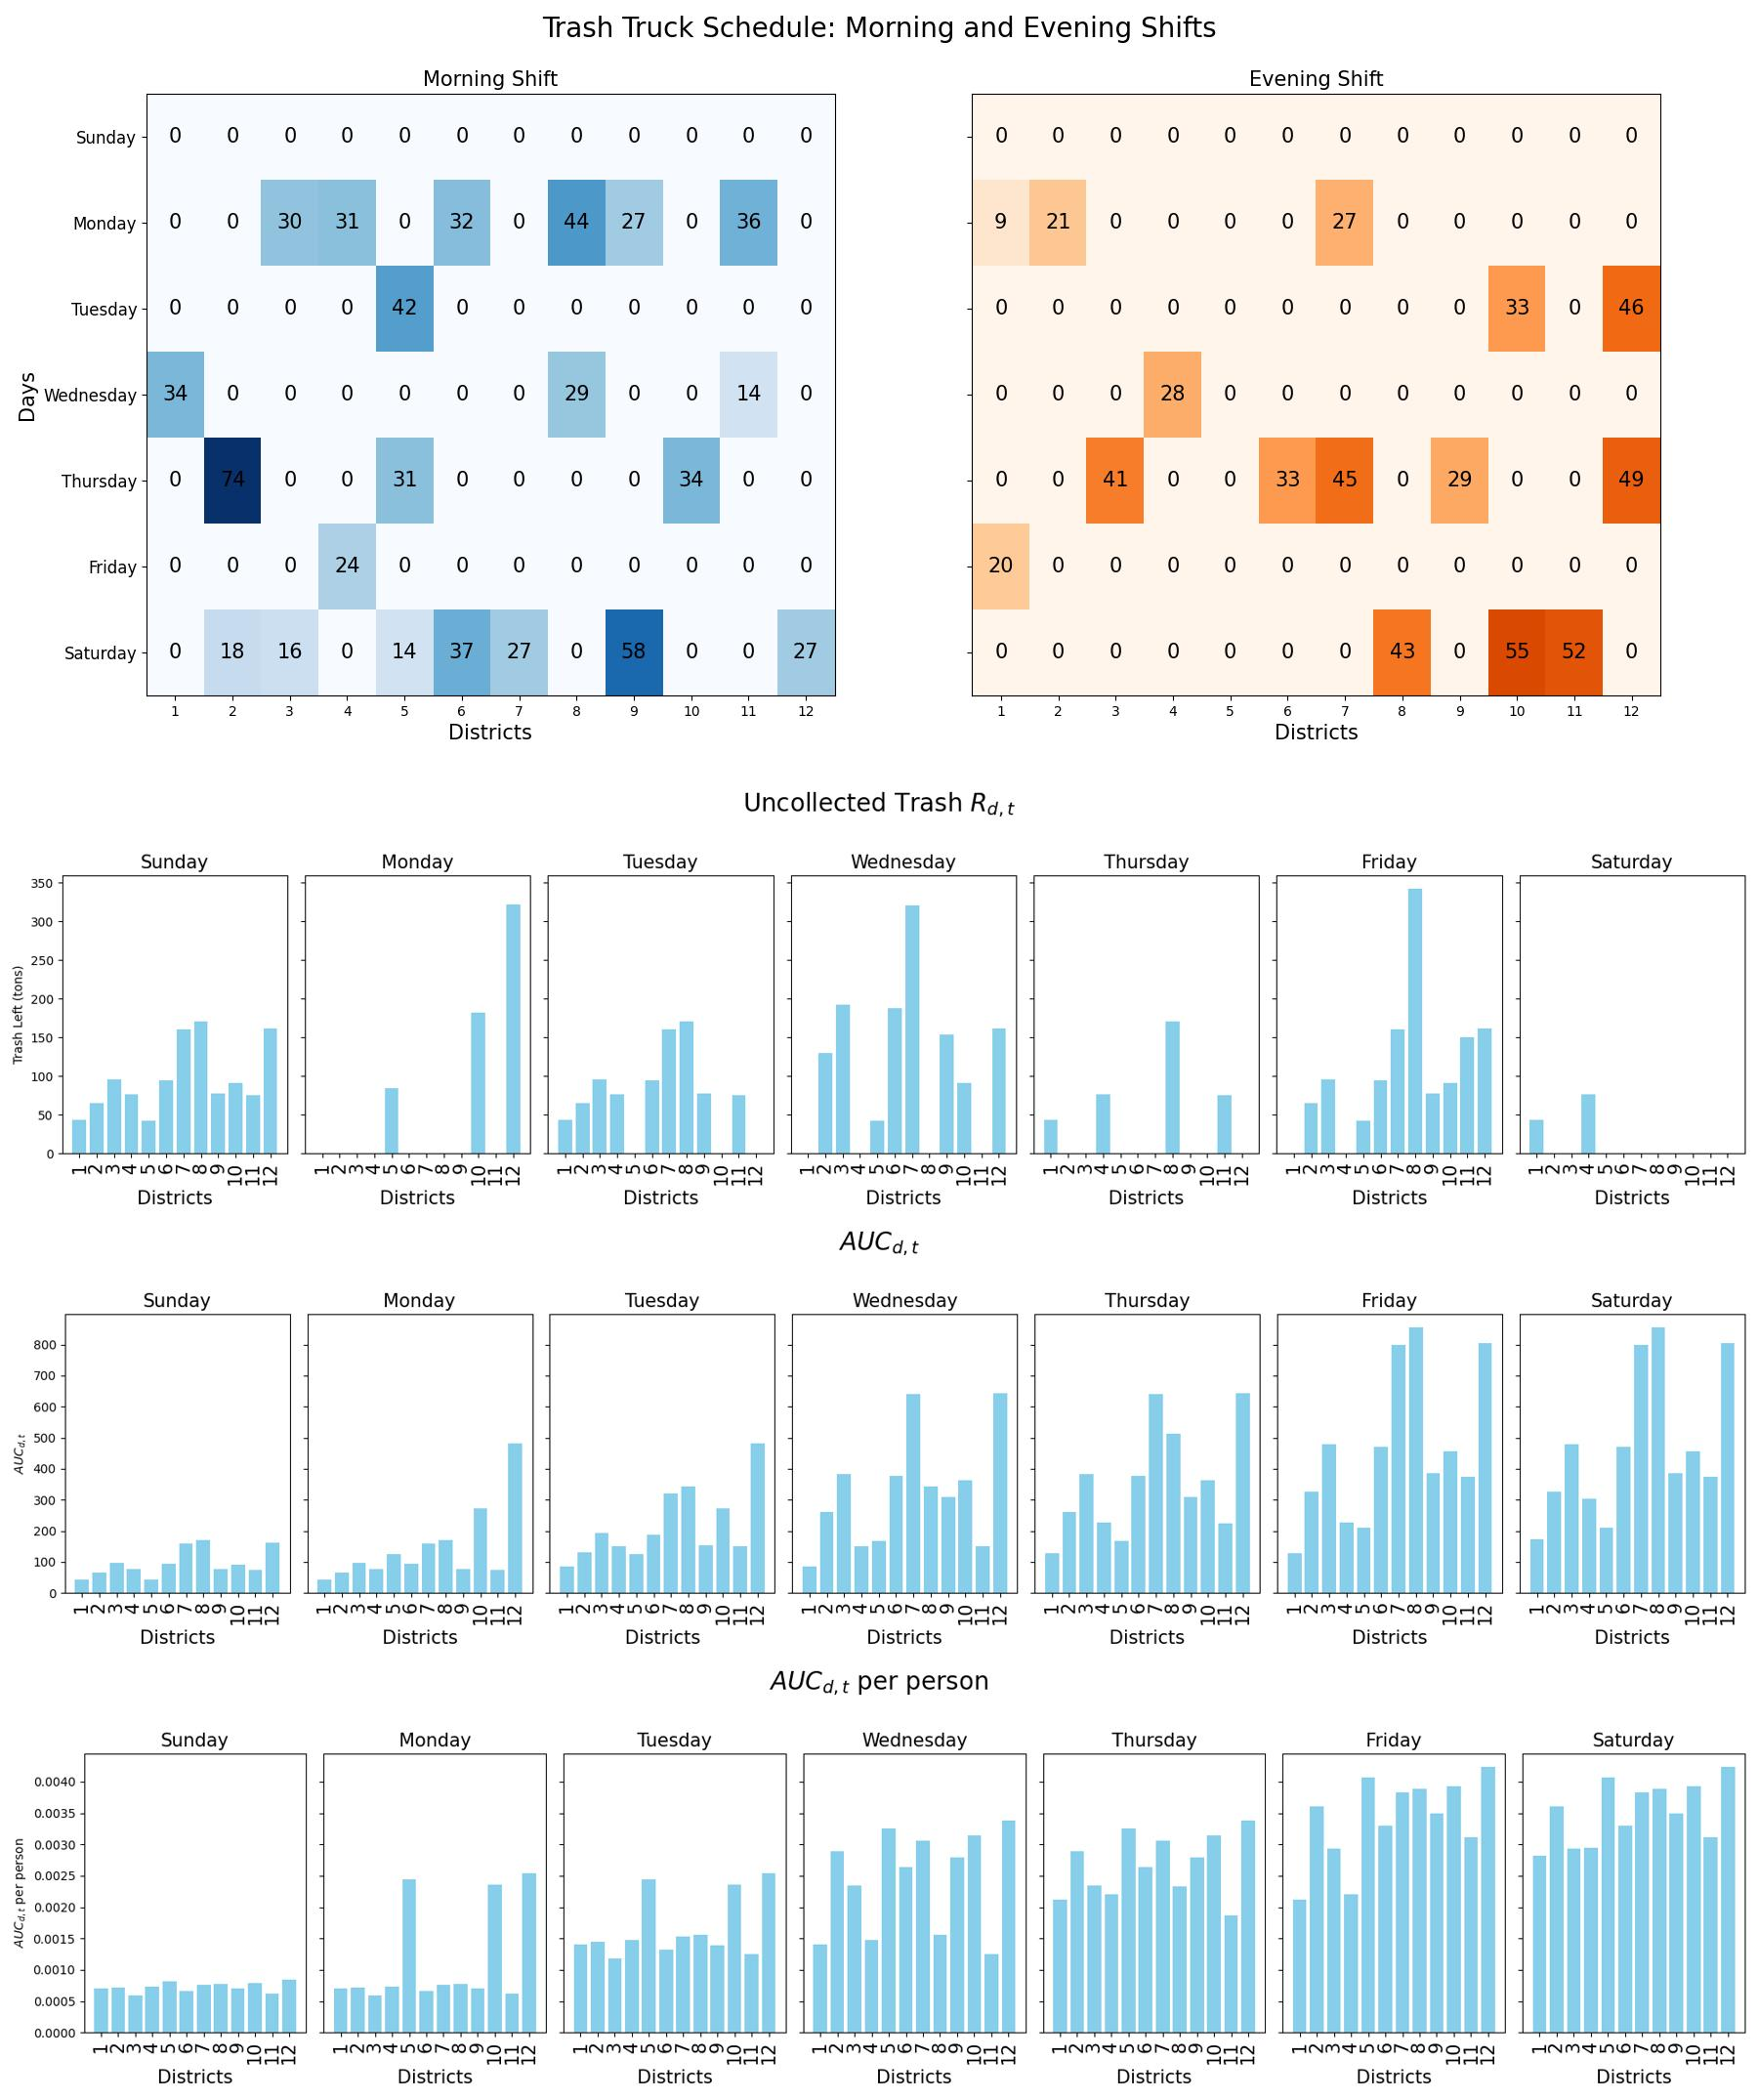
\includegraphics[width=1\textwidth]{figures/(0,1).jpg}
	\caption{Results for $(\lambda_1, \lambda_2) = (0,1)$. ($AUC = 5636.0, E_{eq} = 3.42, E_{ef} = 0.55$). In this case, we prioritize equity and neglect efficiency. We can see visually that the variation of $AUC_{d,t}$ per person on Saturday is lower (lower than, say, \cref{fig:2all}). It is disappointing that unlike the case $(1,0)$, going to an extreme in equity will not result in uniform $AUC_{d,t}$ per person. This is mainly because the 3 time constraint on weekly trash collection guarantees some $AUC$ accumulation, and the districts with higher trash generation rate accumulates more (even averaged out according to population). }
	\label{fig:4all}
\end{figure}


\begin{figure}[H]
	\centering
	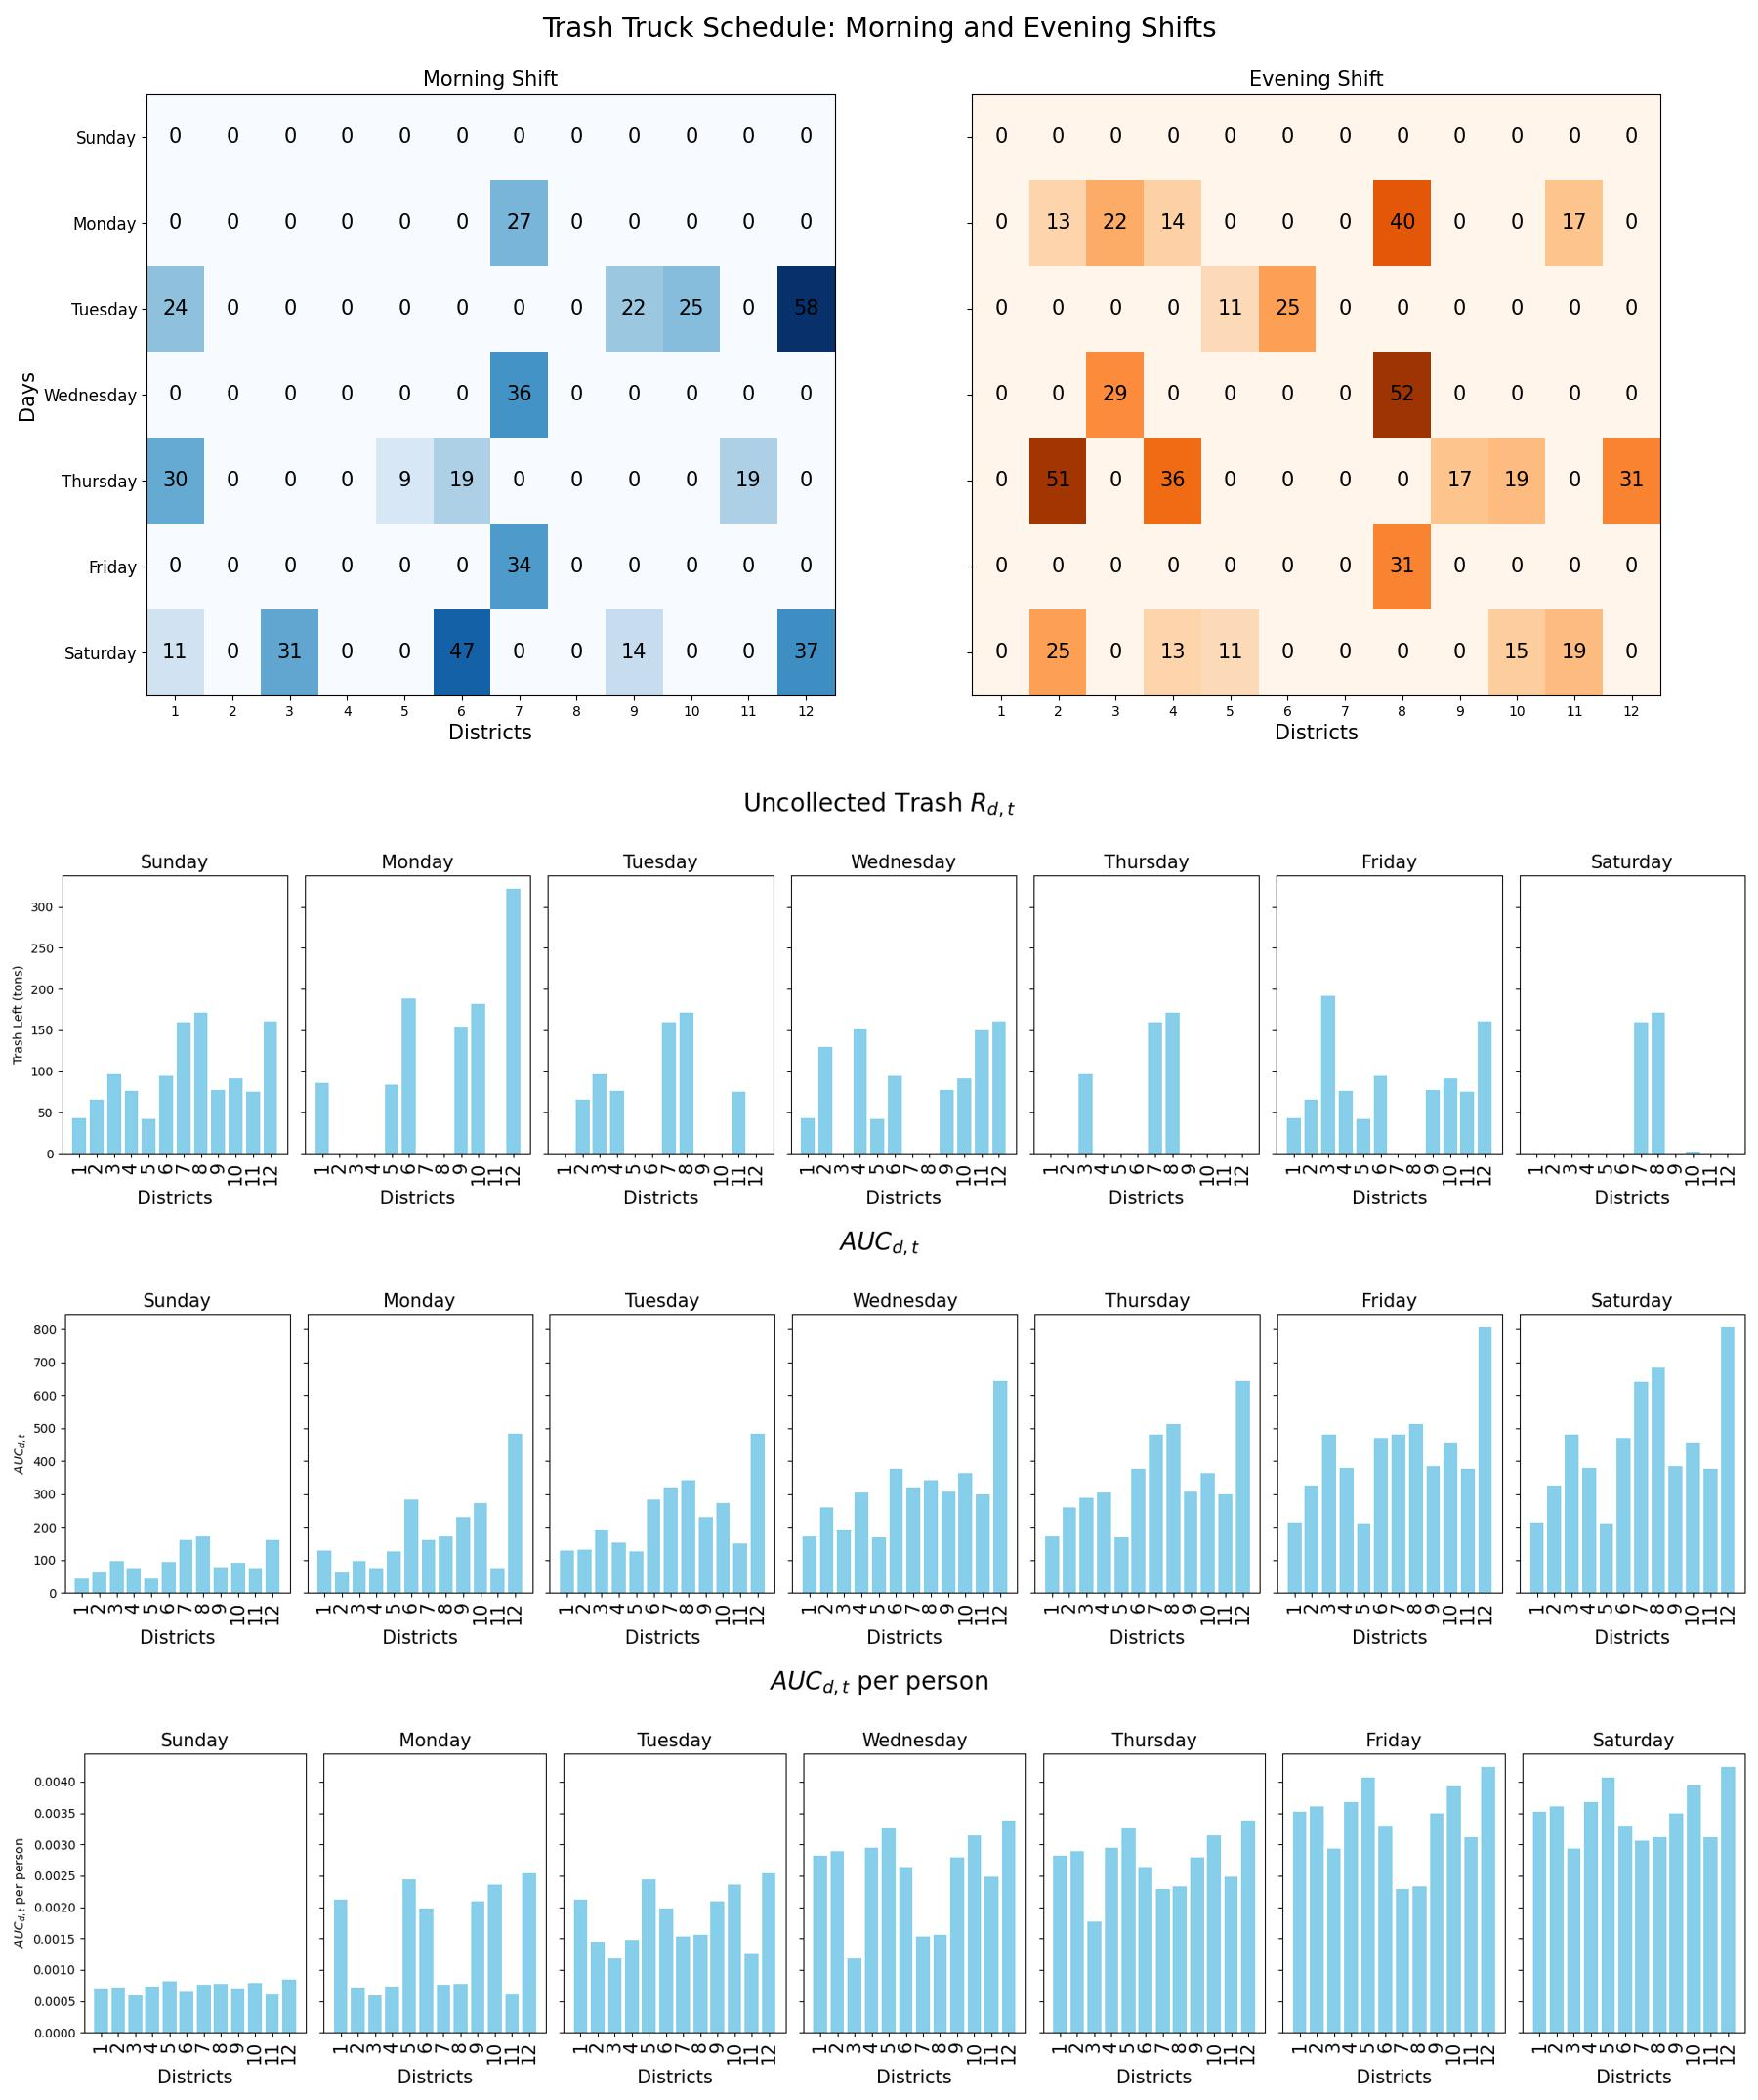
\includegraphics[width=1\textwidth]{figures/(1,1).jpg}
	\caption{Results for $(\lambda_1, \lambda_2) = (1,1)$. ($AUC = 5426.0, E_{eq} = 2.53, E_{ef} = 0.69$). In this case, we try to combine efficiency and equity. Which results in a overall efficiency of 68.92\% and a low variance of $AUC$ per person among different districts. This is the most optimal solution we came about. }
	\label{fig:5all}
\end{figure}
\newpage





\subsection{Comparison With a Real Schedule}

\begin{figure}[H]
	\centering
	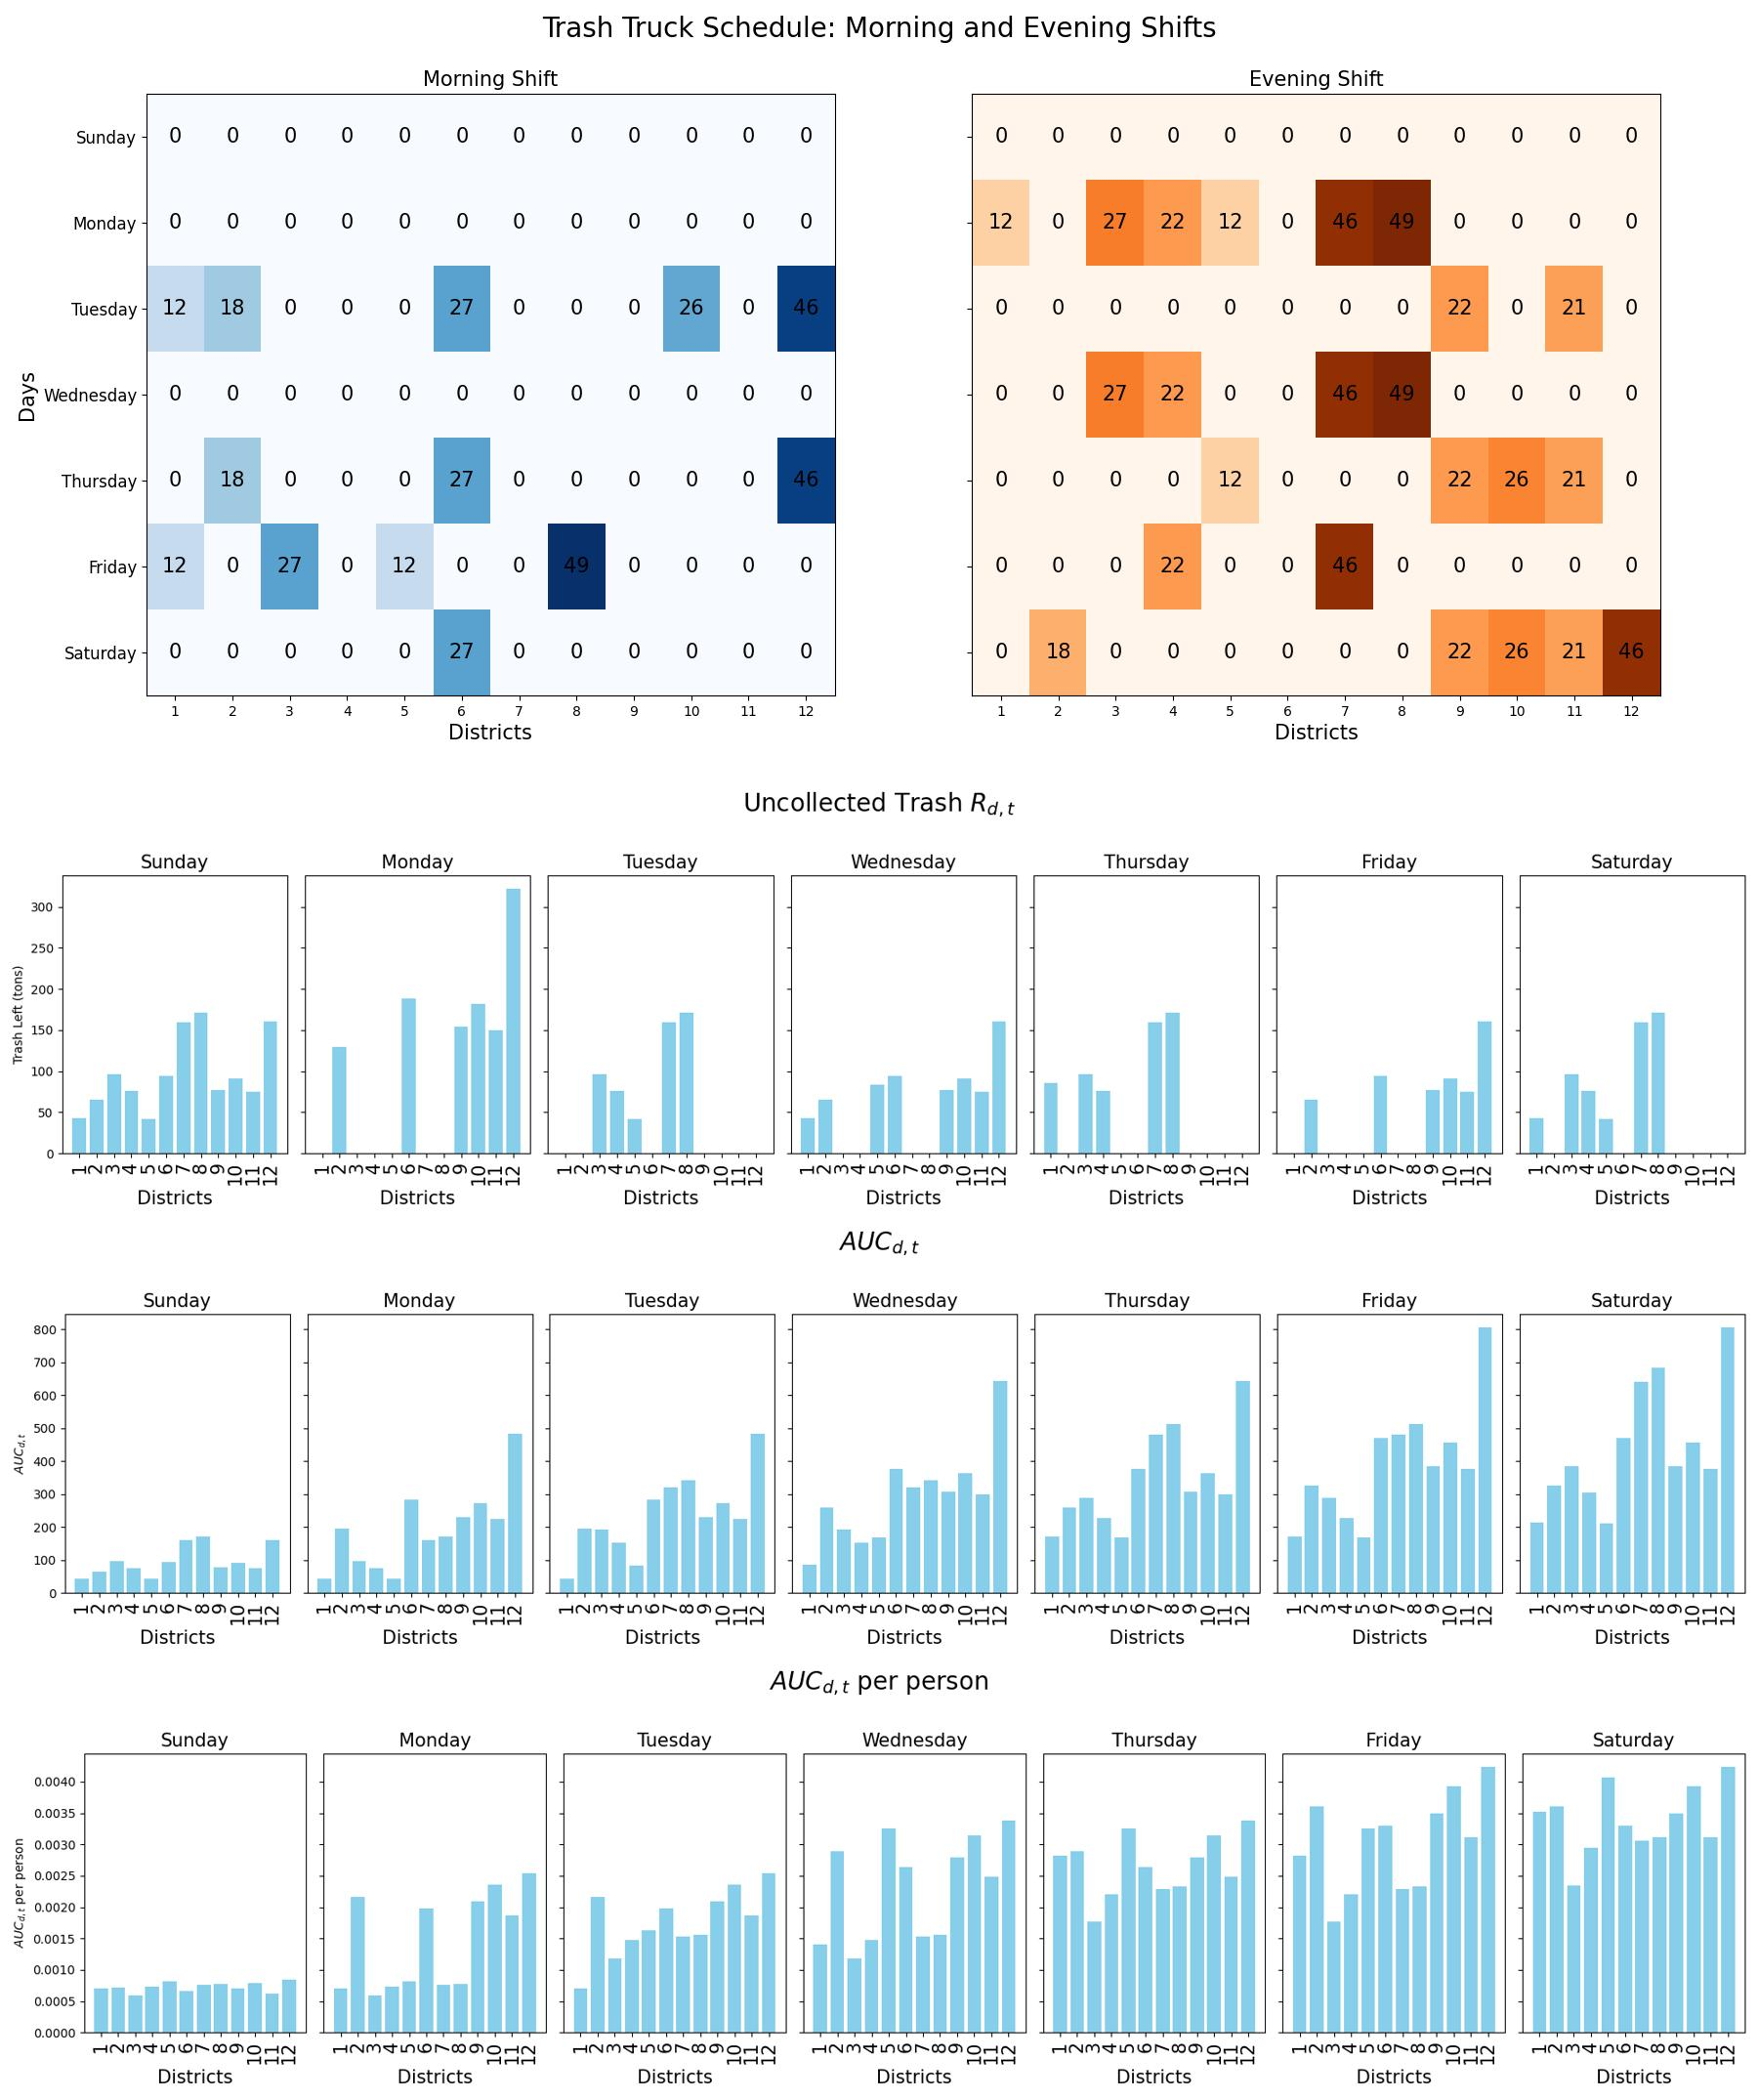
\includegraphics[width=1\textwidth]{figures/Real.jpg}
	\caption{Simulation results for a "real" scenario. ($AUC =  5252.0 $, $E_{eq}= 4.29 ,$ $E_{ef}= 0.63 $).}
	\label{fig:6all}
\end{figure}

Although we do not have detailed information about the trash truck scheduling in reality, the information available is enough for us to make an educated guess. From the data provided,  we do have knowledge about how frequently \cite{Freq} each section of a district is visited. The only unknown piece of information is there number of trucks that where assigned. However, we do have statistical data about the monthly tonnage of each district (\cref{sec:hia}), and trash collected is logically highly proportional to trucks assigned. 

With those assumptions and data in mind, we first let number of trucks we assign to each district be proportional with the monthly tonnage data among districts, and the overall number of trucks roughly equal to the ones we used in the (1,1) AUC solution(\cref{fig:5all}). Next, we picked a random subdistrict for each district, and assign the frequency (i.e. the date of trash collection) of this subdistrict to the district that it belongs to. With this procedure, we arrive at a schedule shown in \cref{fig:6all}.

\begin{table}[H]
\centering
\begin{tabular}{|c|c|c|c|}
\hline
  & $\mathbf{E_{ef}}$ & $\mathbf{E_{eq}}$ & $\mathbf{AUC}$ \\ \hline
$(1,1)$                  & 0.69    & 2.53     & 5426  \\ \hline
"Reality"                & 0.63     & 4.29    & 5252 \\ \hline
\end{tabular}
\caption{Result summary of the AUC model}
\label{tab:optiandreal}
\end{table}


In terms of efficiency and $AUC$, $(1,1)$ and "Reality" are only different marginally, with "Reality" having a slight edge. In terms of equity, $(1,1)$ does perform slightly better, by treating MN3 and MN4 slightly better in terms of $AUC_{d,t}$.

It seems under our assumptions, allocating trucks proportional to trash production is a near optimal choice in the sense of efficiency and $AUC$. On the other hand, the equity factor is not necessaryly optimal for proportional schedules.

\section {Robustness Test} \ 

\label{sec:senana}
To test the robustness of our solution, we used statistical data (See \cref{sec:hia}) to generate random sequences of $W_{d,t}$. By gradually increasing the standard deviation of generated sequence, we evaluate how our solution perform under realistic fluctuations of trash generation. The results are shown in \cref{fig:AUCsen} 

		The generation is achieved by letting:

		\begin{align}
			W_{d,t} \sim \mathcal{N}(m_d, \sigma_d^2)
		\end{align}

		Where $ m_d, \sigma_d^2$ are determined using statistical tonnage data in \cref{sec:hia}. And having $W_{d,t}$ independently generated.


\begin{figure}[H]
	\centering
	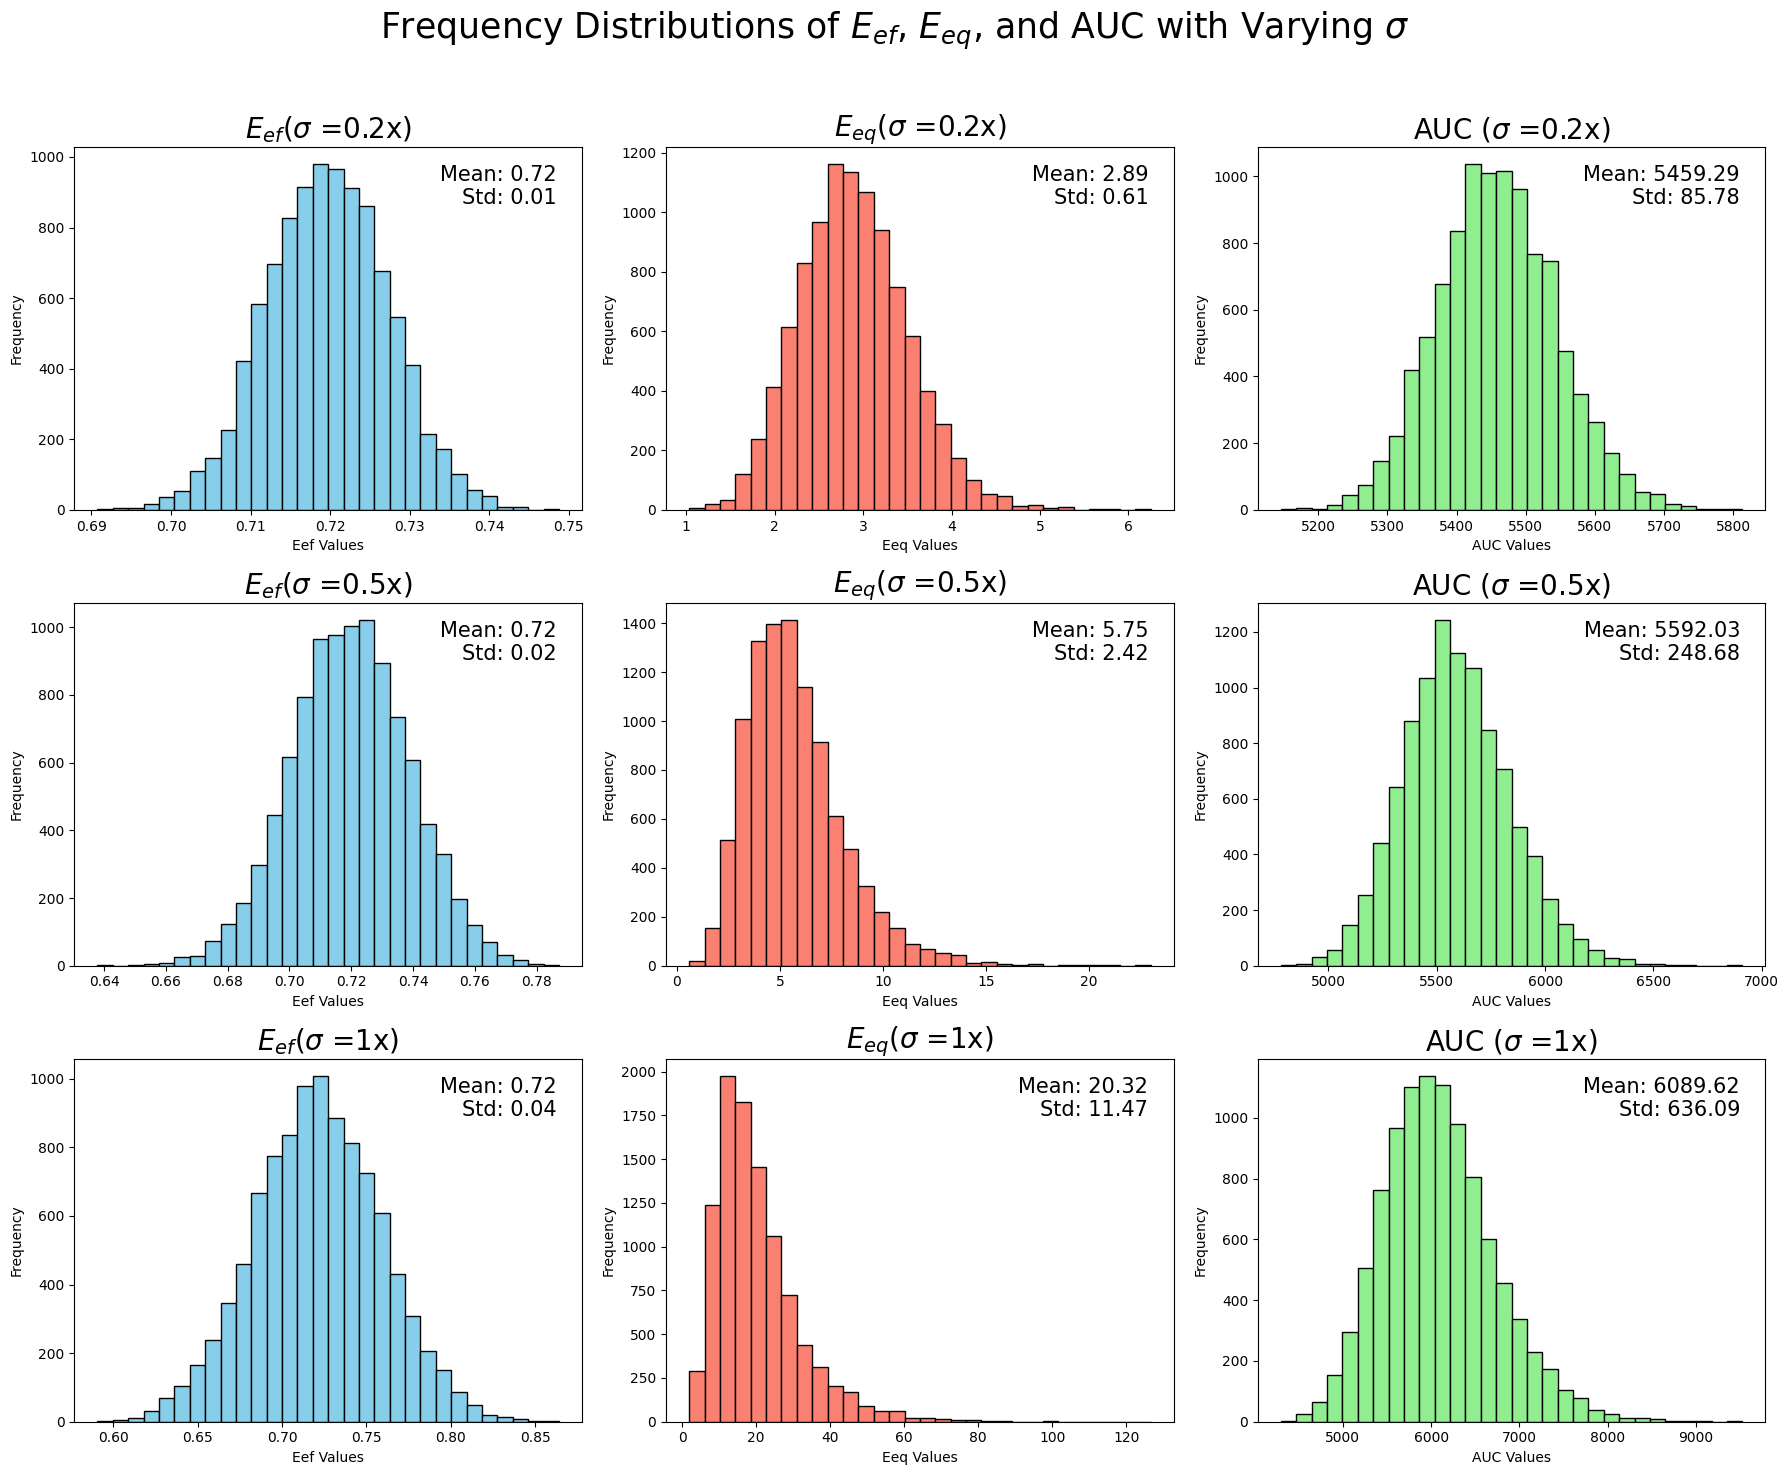
\includegraphics[width=1\textwidth]{figures/rob.png}
	\caption{Sensitivity analysis of the AUC model. We generated 10,000 sets of $ W_{d,t}$ and tested how our solution perform. Where $ \sigma = 0.2x$ denotes $ \sigma = 0.2 \times \sigma_s$, where $ \sigma$ is the standard deviation parameter of the random sequence generation, and $ \sigma_s$ is the statistical value from real world data. 
	From the result we can see that the mean of $ E_{ef} $ and $ AUC$ are not sensitive to the fluctuations of trash generation(where $ E_{ef}$ retained it's mean and $ AUC$ has an 10 \% increase). While the mean of $ E_{eq}$ increased drastically when the transit words real world data happens. This indicates that in real world scenarios, we are not likely to achieve the desired equity of service.   }
	\label{fig:AUCsen}
\end{figure}

From our sensitivity analysis using 10,000 simulated scenarios, we can observe that while our model's performance varies with fluctuating trash output, it maintains reasonably stability in key metrics. Most notably, efficiency ($E_{ef}$) remains remarkably consistent, with the mean value holding steady at 0.72 across all scenarios and the standard deviation only increasing from 0.01 to 0.04 even with 5 times more fluctuation. This suggests our truck utilization remains robust despite input variations.

The equity factor ($E_{eq}$) shows the most sensitivity, with its mean value increasing from 2.88 to 20.32 as variance increases, and standard deviation growing significantly from 0.61 to 13.59. This phenomenon may be tied to the quadratic nature of $E_{eq}$. Also, this result indicates that maintaining equal service levels becomes increasingly challenging with higher trash fluctuations. The AUC shows moderate sensitivity, with the mean value increasing by approximately 10\% (from 5460 to 6093) and standard deviation increasing from 86 to 642, suggesting acceptable degradation in overall performance.

While the decreasing equity metrics might seem concerning, the model maintains its core efficiency and keeps AUC increases manageable even under significant input variance. This suggests that while perfect equity may be harder to achieve in real-world conditions, the model remains practically viable for day-to-day operations, particularly in terms of resource utilization and overall collection performance.

\section{Further Work}

While our models do account for a lot of variables that effect trash pick up, there is definitely room for improvement. Ideally, we want a system that can pick up all trash as mentioned in our model assumptions. However, we understand the infeasibility of such a system, as the system cannot logistically sweep the entire city for all of the trash produced by the residence of the 12 districts; people can forget to take trash out on a designated day, mistakes can be made when it comes to picking up trash on the end of the workers.

\subsection{Static Population Assumption}

Our static population assumption does not account for temporal demographic changes in Manhattan and their impact on waste generation patterns. Also, assuming constant population refrains us from directly using trash tonnage data from the early past, since they are drastically different from now due to the growth of population. Incorporating time series analysis would allow us to evaluate our model's performance under projected population growth scenarios, thereby testing its long-term applicability and robustness.

\subsection{The Advantages of AUC not Apparent}

When we view trash accumulation in the lenses of $AUC$, many quantitative information can be evaluated using analytical methods. Especially with the advancement of modern information technology, the progress made by artificial intelligence and the rapid application of image recognition technology \cite{hossain2019autonomous}, pinpointing every bag of uncollected trash no longer seems impossible. The more granular the data, the more analytical methods reveal their power. We see AUC as a promising means of helping to solve the trash problem for large and complex systems such as metropolises.

\subsection{Deterministic Model requires maximizing the mean proportion of trash collected in 12 districts}

From the results of our deterministic model, the mean proportion of overall trash collected is only around 10\% which is far less than expected. We need to incorporate the mean proportion of trash collected against the total amount of trash generated besides ensuring the equity factor, the variance of mean proportions, is as small as it can be.

\subsection{Complexity of the Deterministic Model's}

Accounting for the activity of each individual truck drastically increases the dimension of the programming problem, which leads to unfeasible amount of solving time. While reducing the dimensions of the problem leads to unrealistic dimensions of the outcome. Putting too many constraint also hinders the existence of solutions. Thus finding a better formulation of the problem is crucial for solving it.


\newpage
\appendix
\section{Historical Information Analysis}
\label{sec:hia}

\begin{figure}[H]
    \centering
    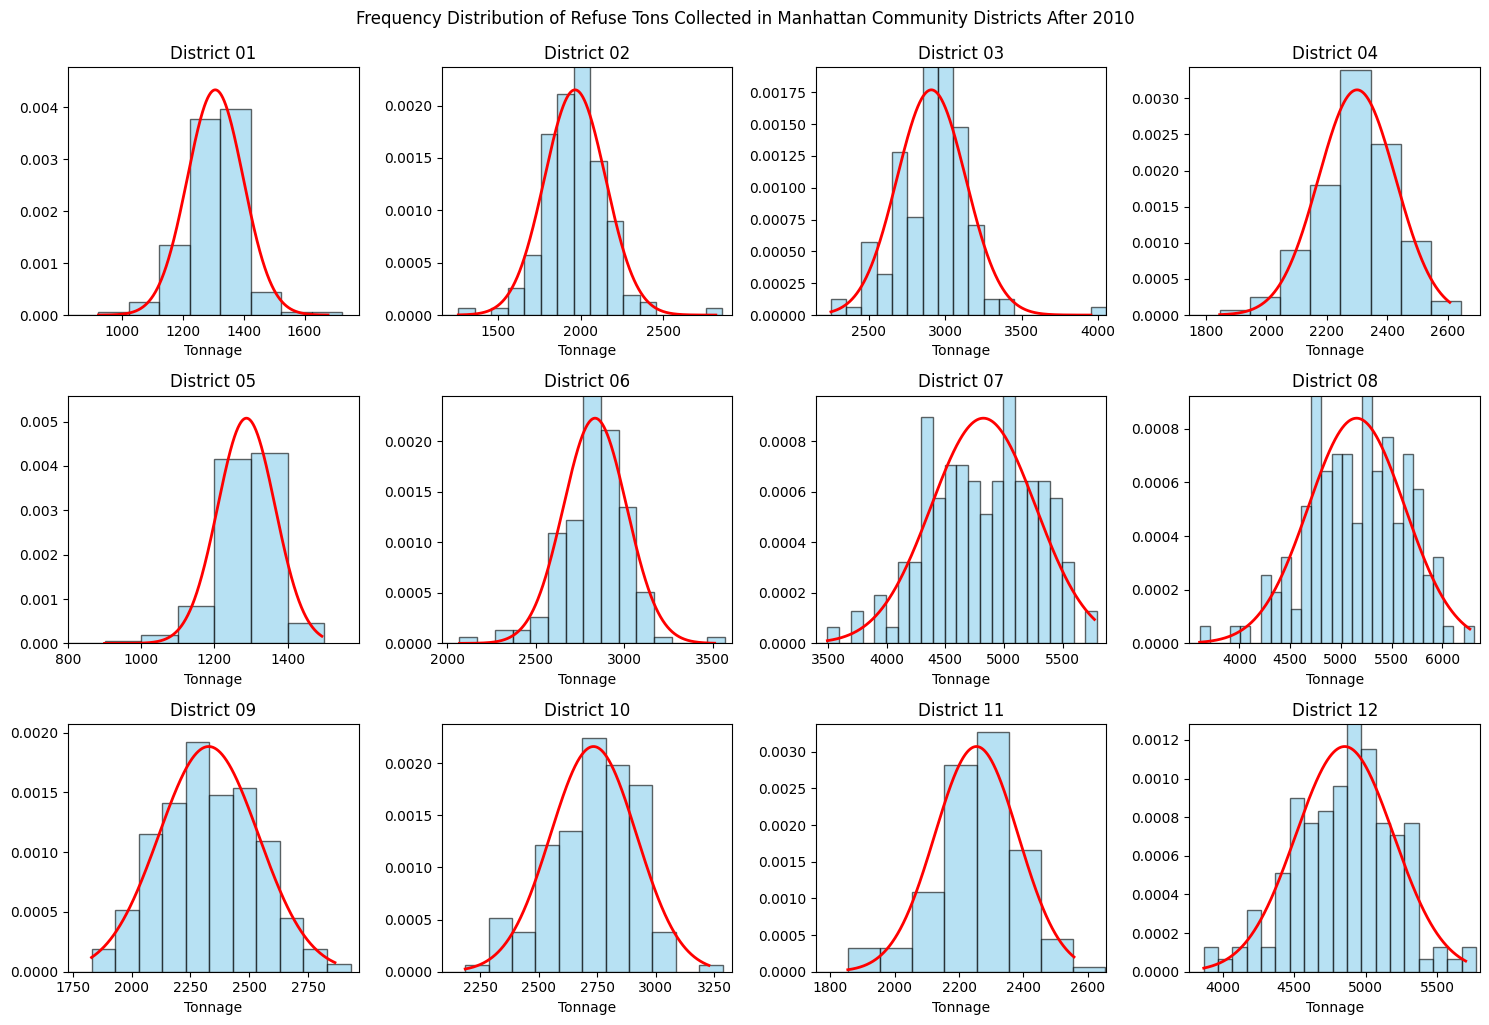
\includegraphics[width=0.9\textwidth]{figures/tonal.png}
	\caption{Monthly tonnage data collected from 2010 to present, considering only refuse trash, fitted with normal distribution }
    \label{fig:tonal}
\end{figure}

We conducted a data cleaning of \cite{MonTon}. Filtering out refuse type trash and year from 2010 to present.

Assuming the monthly tonnage obeys normal distribution, we made a further assumption that the individual days are also independent normal random variables, thus we may calculate the mean and standard deviation of daily trash generation for each district, which is denoted by $(m_d, \sigma_d)$.

\section{Geographic Information Analysis}

As part of determine these models, we performed a considerable amount of data analysis.


The rat heat map is based on the dataset \cite{RatHeat}. While the Daily mean tonnage is from \cref{sec:hia}.

\begin{figure}[H]
    \centering
    \subfigure[Daily mean tonnage collected from 2010 to present]{
        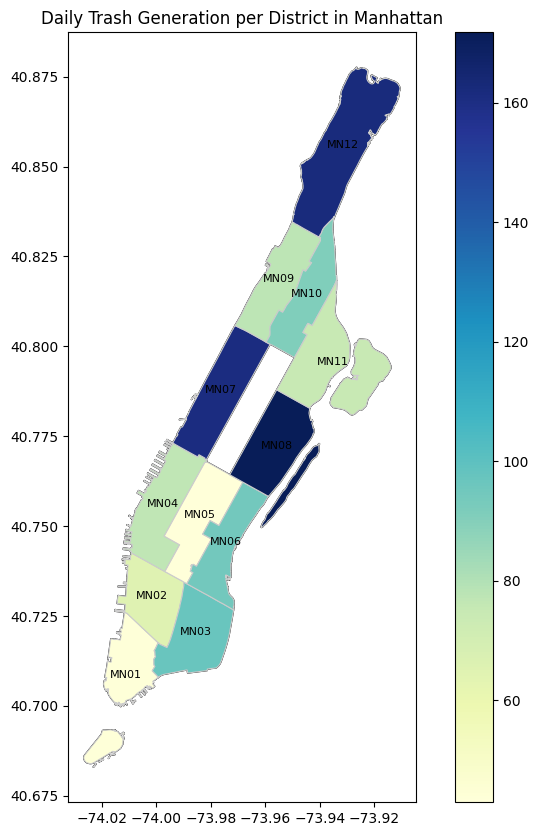
\includegraphics[width=0.46\textwidth]{figures/Estimated_daily_trash_generation.png}
        \label{fig:8first}
    }
    \hfill
    \subfigure[Rat reports in 2010]{
        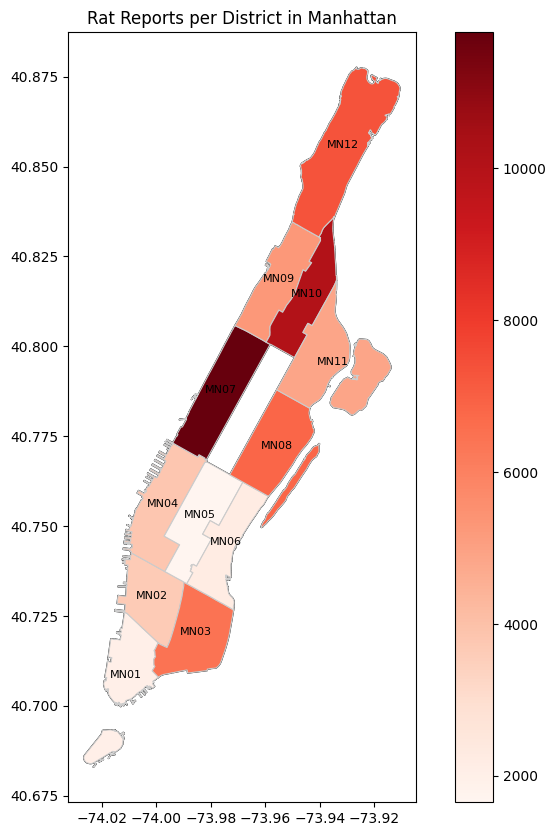
\includegraphics[width=0.47\textwidth]{figures/Rat_report.png}
        \label{fig:8second}
    }
    \caption{Comparison of trash generation (left) and rat reports (right).}
    \label{fig:8both}
\end{figure}

\begin{figure}[H]
	\centering
	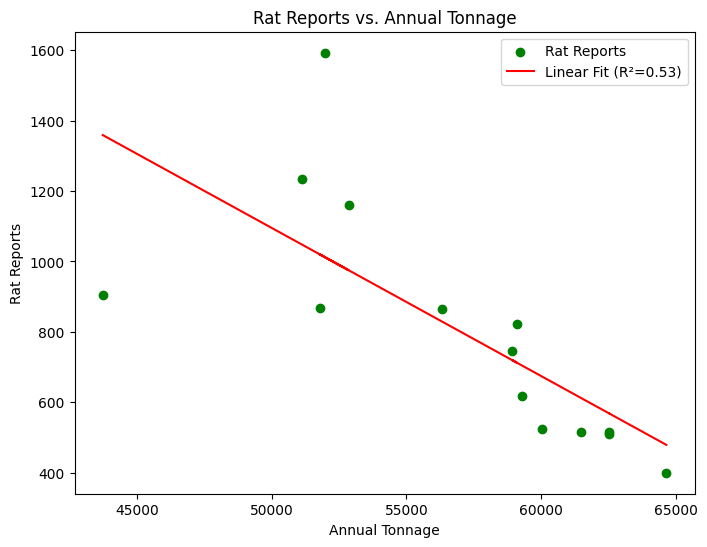
\includegraphics[width=0.9\textwidth]{figures/correlation.png}
	\caption{Scatter plot of mean annual tonnage collected vs. rat reports (2010).}
	\label{fig:9all}
\end{figure}

From \cref{fig:8both} and \cref{fig:9all}, we can clearly see a moderate negative linear correlation (R² = 0.53) between trash collection efficiency and the number of rat reports in a given district. This makes sense; districts with more frequent and efficient trash collection tend to have fewer rat sightings, as there is less available food waste for rats to feed on. This relationship is particularly evident in districts MN07 and MN12, which show high daily trash collection rates in \cref{fig:8first} and correspondingly lower rat reports in Figure \cref{fig:8second}.
However, it's worth noting that this correlation, while significant, explains only about 53\% of the variance in rat reports, suggesting that other factors beyond just trash collection efficiency influence rat populations in Manhattan. These could include:

\begin{itemize}
    \item Building age and infrastructure
    \item Proximity to restaurants and food establishments
    \item Construction activity
    \item Green spaces and parks
    \item Population density
\end{itemize}

This finding reinforces the importance of efficient trash collection not just for cleanliness, but also for public health and pest control considerations.
\newpage
\section{Letter to Head}

To the Head of Waste Management Division at New York City,

We are writing to propose a new system of garbage truck dispersal for districts MN1 to MN12 in the Manhattan borough. As a city that is constantly changing, growing in population, and experiencing widening socioeconomic gaps, we believe that implementing a more dynamic schedule is essential for optimizing waste management operations.

Our comprehensive analysis has led to the development of a Area-Under-Curve (AUC) Model that optimally balances efficiency with equity. This model achieves a 68.92\% efficiency rate in truck utilization while requiring only 223 trucks maximum per day (versus the current 2,230 available) and reduces weekly uncollected waste from 588 tons to 276 tons across Manhattan. The model incorporates critical factors including socioeconomic indicators, population density, and district-specific waste generation patterns to create a more equitable and efficient collection system. Our innovative approach considers not just the amount of waste collected, but also how long waste remains uncollected in each district, ensuring both operational efficiency and community satisfaction. Below is our proposed AUC model schedule in a concise table.

\begin{table}[H]
\centering
\begin{tabular}{|l|l|l|l|l|l|l|l|}
\hline
District & Sunday & Monday & Tuesday & Wednesday & Thursday & Friday & Saturday \\ \hline
MN1 & - & - & M(24) & - & M(30) & - & M(11) \\ \hline
MN2 & - & - & - & - & E(51) & - & E(25) \\ \hline
MN3 & - & - & - & E(29) & - & - & M(31) \\ \hline
MN4 & - & E(14) & - & - & E(36) & - & E(13) \\ \hline
MN5 & - & - & - & - & M(9) & - & E(11) \\ \hline
MN6 & - & - & E(25) & - & M(19) & - & M(47) \\ \hline
MN7 & - & M(27) & - & M(36) & - & M(34) & - \\ \hline
MN8 & - & E(40) & - & E(52) & - & E(31) & - \\ \hline
MN9 & - & - & M(22) & - & - & - & M(14) \\ \hline
MN10 & - & - & M(25) & - & E(19) & - & E(15) \\ \hline
MN11 & - & E(17) & - & - & M(19) & - & E(19) \\ \hline
MN12 & - & - & M(58) & - & E(31) & - & M(37) \\ \hline
\textbf{Total} & \textbf{0} & \textbf{98} & \textbf{154} & \textbf{117} & \textbf{214} & \textbf{65} & \textbf{223} \\ \hline
\end{tabular}
\label{tab:schedule}
\caption*{Weekly Garbage Collection Schedule by District. M = Morning shift (7 AM-8 AM), E = Evening shift (6 PM - 7 PM), numbers in parentheses indicate number of trucks assigned.}
\end{table}

However, we acknowledge several limitations that require careful consideration. Our equity metrics show increased sensitivity under real-world conditions, suggesting the need for implementing monitoring systems to identify and address service gaps. The model's AUC (which indicates the environmental and social impact of uncollected trash) shows moderate sensitivity to input variations, with approximately 10\% increase under scenarios where trash demand fluctuates. Additionally, our current model is derived under constant waste generation assumptions, not accounting for seasonal variations. We recommend quarterly schedule adjustments to address these fluctuations. The implementation complexity will require significant changes to current routing systems, and we suggest a phased implementation starting with pilot districts.

To move forward, we need to establish methods for discussing with managers, workers, and stakeholders in this new change, conduct further cost-benefit analysis and assess technology infrastructure needs. Our analysis demonstrates that this new approach could significantly improve Manhattan's waste management efficiency while better serving our diverse communities. We welcome the opportunity to discuss these recommendations in detail and develop an implementation strategy that aligns with your operational capabilities.

Respectfully submitted,

Ethan Carlson, Xieqing Yu, and Yuanqi Yu


\section{Other Geological Factors}

\begin{figure}[H]
	\centering
	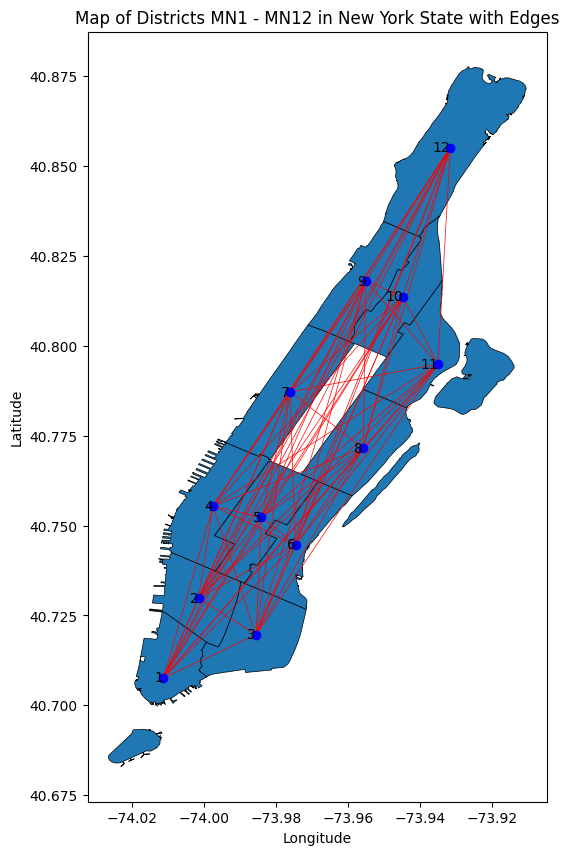
\includegraphics[width=0.9\textwidth]{figures/linemap.png}
	\caption{Map representation of all district connections for our models}
	\label{fig:10all}
\end{figure}

\begin{figure}[H]
	\centering
	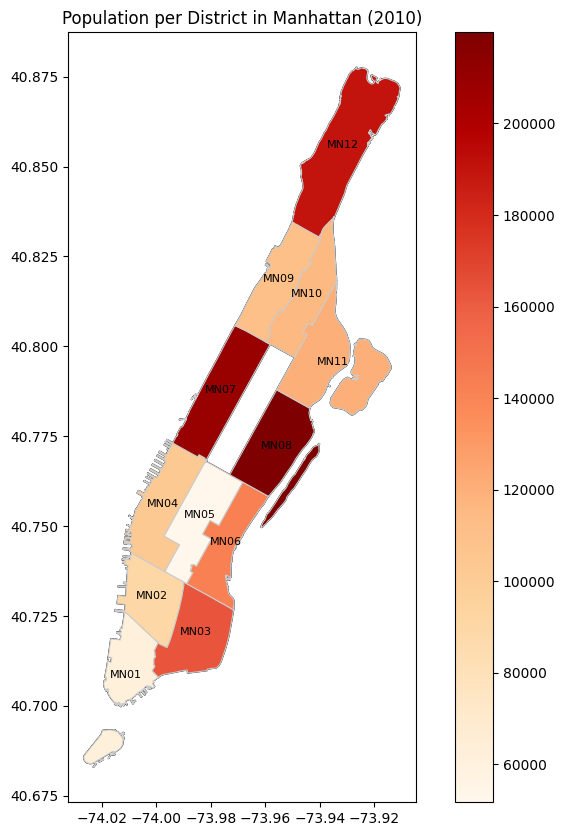
\includegraphics[width=0.9\textwidth]{figures/population.png}
	\caption{Map representation of populations totals in 2010}
	\label{fig:11all}
\end{figure}

\section{Python Code}
\subsection{Deterministic Model}
\subsubsection{Fixed Assignment Model}

\begin{minted}[breaklines=true]{python}

import pulp as lp
import random

# Parameters
districts = range(12)  # 12 districts
days = range(7)  # Days in a week
timeslots = ["Morning", "Evening"]  # Two timeslots
total_trucks = 500  # Adjusted for feasibility
truck_capacity = 12  # Each truck’s capacity in tons
truck_collection_time_per_ton = 1  # Collection time per ton (for simplicity)
alpha = 1.0  # Weight for TCT
gamma = 1.0  # Weight for PGC
beta = 1.0  # Weight for TGC

lower_limit = [27, 32, 56, 53, 29, 62, 79, 85, 39, 57, 51, 99]
upper_limit = [60, 99, 138, 100, 57, 127, 243, 259, 116, 125, 99, 224]

# Randomly generated data
waste_generated = {d: {day: random.uniform(lower_limit[d], upper_limit[d]) for day in days} for d in districts}
# {d: {day: random.uniform(5, 25) for day in days} for d in districts}
frequency_required = {d: random.choice([2, 3]) for d in districts}
SEI = {d: random.uniform(0, 1) for d in districts}

# Initialize Model
model_fixed = lp.LpProblem("Fixed_Assignment_Model", lp.LpMinimize)

# Decision variables: binary and non-negative
x_fixed = lp.LpVariable.dicts("x_fixed", ((d, t, k, day) for d in districts for t in range(total_trucks)
                                          for k in timeslots for day in days), 0, 1, lp.LpBinary)
# Decision variable: y_shared_new = 1 if truck t is assigned to district d for any timeslot in a week
y_shared_new = lp.LpVariable.dicts("y_shared_new",
                                   ((d, t) for d in districts for t in range(total_trucks)), 0, 1, lp.LpBinary)
g_fixed = lp.LpVariable.dicts("g_fixed", ((d, day) for d in districts for day in days), 0)  # Non-negative variable

proportions = []

# Loop over each district to compute the collected/generated ratio
for d in districts:
    # Total waste generated by district d
    total_waste_generated_d = sum(waste_generated[d][day] for day in days)

    # Total garbage collected for district d across all days
    total_garbage_collected_d = lp.lpSum(g_fixed[(d, day)] for day in days)

    # Calculate ratio if total waste generated is non-zero
    if total_waste_generated_d != 0:
        ratio = total_garbage_collected_d / total_waste_generated_d
        proportions.append(ratio)

# Linear approximation using absolute deviations from mean
# Auxiliary variable to represent the mean of proportions
mean_proportion = lp.LpVariable("mean_proportion", lowBound=0)

# Add constraint for mean calculation
model_fixed += (mean_proportion == lp.lpSum(proportions) / len(proportions))

# List to hold absolute deviations
abs_deviations = []

for i, proportion in enumerate(proportions):
    # Auxiliary variables for positive and negative deviations
    pos_dev = lp.LpVariable(f"pos_dev_{i}", lowBound=0)
    neg_dev = lp.LpVariable(f"neg_dev_{i}", lowBound=0)

    # Constraint to express absolute deviation from mean
    model_fixed += (proportion - mean_proportion == pos_dev - neg_dev, f"Deviation_{i}")

    # Add positive and negative deviations to get the absolute deviation
    abs_deviation = pos_dev + neg_dev
    abs_deviations.append(abs_deviation)


# Objective functions
def TCT(x):
    return lp.lpSum(x[(d, t, k, day)] * truck_collection_time_per_ton * truck_capacity for d in districts for t in
                    range(total_trucks) for k in timeslots for day in days)


def TGC(g):
    return lp.lpSum(g[(d, day)] for d in districts for day in days)


# Define an objective function that includes minimizing absolute deviations
model_fixed += alpha * TCT(x_fixed) - beta * TGC(g_fixed) + gamma * (lp.lpSum(abs_deviations) / len(proportions))

# Constraints
for d in districts:
    for day in days:
        # Garbage collection constraints
        model_fixed += g_fixed[(d, day)] == lp.lpSum(
            x_fixed[(d, t, k, day)] * truck_capacity for t in range(total_trucks) for k in
            timeslots), f"GarbageCollection_Fixed_{d}_{day}"

# Step 1: Create a binary variable to track if a schedule (day, timeslot) is used in a district
schedule_used = lp.LpVariable.dicts("schedule_used",
                                    ((d, day, k) for d in districts for day in days for k in timeslots),
                                    0, 1, lp.LpBinary)

# Step 2: Set schedule_used to 1 if any truck is assigned to a district on a given (day, timeslot)
for d in districts:
    for day in days:
        for k in timeslots:
            # Upper bound constraint
            model_fixed += schedule_used[(d, day, k)] <= lp.lpSum(
                x_fixed[(d, t, k, day)] for t in range(total_trucks)), f"ScheduleUsed_Upper_{d}_{day}_{k}"

            # Lower bound constraint
            model_fixed += lp.lpSum(x_fixed[(d, t, k, day)] for t in range(total_trucks)) <= schedule_used[
                (d, day, k)] * total_trucks, f"ScheduleUsed_Lower_{d}_{day}_{k}"

# Step 3: Limit the total number of distinct schedules to 2 or 3 for each district
for d in districts:
    model_fixed += lp.lpSum(schedule_used[(d, day, k)] for day in days for k in timeslots) >= 2, f"MinSchedules_{d}"
    model_fixed += lp.lpSum(schedule_used[(d, day, k)] for day in days for k in timeslots) <= 3, f"MaxSchedules_{d}"

# Additional binary variable to indicate if a truck is assigned to a district at all
z = lp.LpVariable.dicts("z", ((t, d) for t in range(total_trucks) for d in districts), 0, 1, lp.LpBinary)

# Link x_fixed and z variables
for t in range(total_trucks):
    for d in districts:
        # Link x_fixed and z: if z[t, d] is 1, truck t can be assigned to district d on specific (day, timeslot) combinations
        model_fixed += lp.lpSum(x_fixed[(d, t, k, day)] for day in days for k in timeslots) <= z[(t, d)] * len(
            days) * len(timeslots)

# Ensure each truck is assigned to exactly one district across all days and timeslots
for t in range(total_trucks):
    model_fixed += lp.lpSum(z[(t, d)] for d in districts) == 1, f"OneDistrictP#_{t}"

# Solve the model
model_fixed.solve(lp.PULP_CBC_CMD(msg=1, timeLimit=100))

# Display results
print("Fixed Assignment Model:")
print("Status:", lp.LpStatus[model_fixed.status])
print("Objective Value:", lp.value(model_fixed.objective))

# Output assignment results for diagnostics
for d in districts:
    for day in days:
        for t in range(total_trucks):
            for k in timeslots:
                if lp.value(x_fixed[(d, t, k, day)]) > 0:
                    print(f"District {d}, Truck {t}, {k}, Day {day}: Assignment = {lp.value(x_fixed[(d, t, k, day)])}")

# Compute TCT (Total Collection Time)
TCT = sum(x[d,t,k,day].varValue * truck_collection_time_per_ton * truck_capacity for d in districts for t in total_trucks for k in timeslots for day in days)

# Compute TGC (Total Garbage Collected)
TGC = sum(g[d,day].varValue for d in districts for day in days)

# Compute PGC (Proportional Garbage Collection)
PGC = sum(abs_deviations[i].varValue for i in range(1, len(districts)+1)) / len(districts)

# Output the values
print(f"Total Collection Time (TCT): {TCT}")
print(f"Total Garbage Collected (TGC): {TGC}")
print(f"Proportional Garbage Collection (PGC): {PGC}")

\end{minted}

\subsubsection{Truck Sharing model}

\begin{minted}[breaklines=true]{python}

import pulp as lp
import random

# Parameters
districts, days = range(12), range(7)
timeslots, total_trucks = ["Morning", "Evening"], 500
truck_capacity, alpha, beta, gamma = 12, 1.0, 1.0, 1.0
lower_limit = [27, 32, 56, 53, 29, 62, 79, 85, 39, 57, 51, 99]
upper_limit = [60, 99, 138, 100, 57, 127, 243, 259, 116, 125, 99, 224]
random.seed(42)

# Random data
waste_generated = {d: {day: random.uniform(lower_limit[d], upper_limit[d]) for day in days} for d in districts}
frequency_required = {d: random.choice([2, 3]) for d in districts}
SEI = {d: random.uniform(0, 1) for d in districts}

# Model and decision variables
model = lp.LpProblem("Truck_Shared_Model", lp.LpMinimize)
x_shared = lp.LpVariable.dicts("x", ((d, t, k, day) for d in districts for t in range(total_trucks)
                                     for k in timeslots for day in days), 0, 1, lp.LpBinary)
g_shared = lp.LpVariable.dicts("g", ((d, day) for d in districts for day in days), 0)
proportions = []

# Compute collected/generated ratio per district
for d in districts:
    total_waste = sum(waste_generated[d][day] for day in days)
    total_collected = lp.lpSum(g_shared[(d, day)] for day in days)
    if total_waste != 0:
        proportions.append(total_collected / total_waste)

# Mean proportion and deviations
mean_proportion = lp.LpVariable("mean_proportion", lowBound=0)
model += mean_proportion == lp.lpSum(proportions) / len(proportions)
abs_deviations = []
for i, p in enumerate(proportions):
    pos_dev, neg_dev = lp.LpVariable(f"pos_dev_{i}", 0), lp.LpVariable(f"neg_dev_{i}", 0)
    model += (p - mean_proportion == pos_dev - neg_dev)
    abs_deviations.append(pos_dev + neg_dev)

# Objective functions
def TCT(x): return lp.lpSum(x[(d, t, k, day)] * truck_capacity for d in districts for t in range(total_trucks)
                            for k in timeslots for day in days)
def TGC(g): return lp.lpSum(g[(d, day)] for d in districts for day in days)

model += alpha * TCT(x_shared) - beta * TGC(g_shared) + gamma * (lp.lpSum(abs_deviations) / len(proportions))

# Constraints
for d in districts:
    for day in days:
        model += g_shared[(d, day)] == lp.lpSum(x_shared[(d, t, k, day)] * truck_capacity
                                                for t in range(total_trucks) for k in timeslots)

schedule_used = lp.LpVariable.dicts("schedule_used", ((d, day, k) for d in districts for day in days for k in timeslots), 0, 1, lp.LpBinary)

for d in districts:
    for day in days:
        for k in timeslots:
            model += schedule_used[(d, day, k)] <= lp.lpSum(x_shared[(d, t, k, day)] for t in range(total_trucks))
            model += lp.lpSum(x_shared[(d, t, k, day)] for t in range(total_trucks)) <= schedule_used[(d, day, k)] * total_trucks

for d in districts:
    model += 2 <= lp.lpSum(schedule_used[(d, day, k)] for day in days for k in timeslots) <= 3

for t in range(total_trucks):
    for day in days:
        for k in timeslots:
            model += lp.lpSum(x_shared[(d, t, k, day)] for d in districts) <= 1

# Solve and display results
model.solve(lp.PULP_CBC_CMD(msg=1, timeLimit=100))
print("Truck Sharing Model Status:", lp.LpStatus[model.status])
print("Objective Value:", lp.value(model.objective))

for d in districts:
    for day in days:
        for t in range(total_trucks):
            for k in timeslots:
                if lp.value(x_shared[(d, t, k, day)]) > 0:
                    print(f"District {d}, Truck {t}, {k}, Day {day}: Assignment = {lp.value(x_shared[(d, t, k, day)])}")

# Compute TCT (Total Collection Time)
TCT = sum(x[d,t,k,day].varValue * truck_collection_time_per_ton * truck_capacity for d in districts for t in total_trucks for k in timeslots for day in days)

# Compute TGC (Total Garbage Collected)
TGC = sum(g[d,day].varValue for d in districts for day in days)

# Compute PGC (Proportional Garbage Collection)
PGC = sum(abs_deviations[i].varValue for i in range(1, len(districts)+1)) / len(districts)

# Output the values
print(f"Total Collection Time (TCT): {TCT}")
print(f"Total Garbage Collected (TGC): {TGC}")
print(f"Proportional Garbage Collection (PGC): {PGC}")

\end{minted}


\subsection{AUC Model}

\begin{minted}[breaklines=true]{python}

import pickle
import numpy as np
import matplotlib.pyplot as plt
from joblib import Parallel, delayed
import os




def plot_week_data(daily_trash_data, y_label, title, filename=None):
    """
    Plots the remaining trash for each district across all 7 days and optionally saves the plot to a file.
    
    Parameters:
    - daily_trash_data: 3D numpy array containing trash data in the form (days, districts, 2),
                        where the third dimension holds [remaining_trash, accumulated_trash_delay].
    - y_label: Label for the y-axis.
    - title: Title of the plot.
    - filename: Optional; if provided, the plot will be saved to this file.
    """
    days = daily_trash_data.shape[0]
    districts = daily_trash_data.shape[1]
    day_names = ["Sunday", "Monday", "Tuesday", "Wednesday", "Thursday", "Friday", "Saturday"]
    
    # Set up the figure with subplots for each day
    fig, axs = plt.subplots(1, days, figsize=(20, 5), sharey=True)
    fig.suptitle(title, fontsize=20)
    
    # Loop over each day and plot the remaining trash for all districts
    for day in range(days):
        remaining_trash = daily_trash_data[day, :]  # Extract remaining trash for all districts on the given day
        axs[day].bar(range(districts), remaining_trash, color='skyblue')
        axs[day].set_title(day_names[day], fontsize=15)  # Set title to day name
        axs[day].set_xlabel('Districts', fontsize=15)
        axs[day].set_xticks(range(districts))
        axs[day].set_xticklabels([f'{i+1}' for i in range(districts)], rotation=90, fontsize=15)
    
    axs[0].set_ylabel(y_label)
    plt.tight_layout(rect=[0, 0, 1, 0.96])  # Adjust layout to fit the title

    # Save the plot if a filename is provided
    if filename:
        plt.savefig(filename)
    
    plt.show()


def calculate_trash_delay(daily_trash_data):
    days = daily_trash_data.shape[0]
    districts = daily_trash_data.shape[1]
    
    # Calculate cumulative accumulated trash delay over the week
    cumulative_trash_delay = np.zeros((days, districts))
    cumulative_trash_delay[0] = daily_trash_data[0, :, 1]  # Initialize with the first day's accumulated delay
    
    for day in range(1, days):
        cumulative_trash_delay[day] = cumulative_trash_delay[day - 1] + daily_trash_data[day, :, 1]  # Add previous day's delay
    
    return cumulative_trash_delay[day]

def plot_truck_schedule(schedule, filename=None):
    """
    Visualizes the truck schedule over a week with two subplots for morning and evening shifts,
    displaying the number of trucks in each cell centered and adding color to indicate quantities.
    
    Parameters:
    - schedule: 3D numpy array with shape (12, 7, 2) where schedule[i][j][k] represents
                the number of trucks sent to district i on day j in shift k (0 for morning, 1 for evening).
    - filename: Optional; if provided, the plot will be saved to this file.
    """
    days, districts = schedule.shape[1], schedule.shape[0]
    day_names = ["Sunday", "Monday", "Tuesday", "Wednesday", "Thursday", "Friday", "Saturday"]

    # Extract morning and evening schedules
    morning_schedule = schedule[:, :, 0].T  # Transpose for 7x12 display
    evening_schedule = schedule[:, :, 1].T  # Transpose for 7x12 display

    # Set up the figure with two subplots
    fig, axs = plt.subplots(1, 2, figsize=(20, 8), sharey=True)
    fig.suptitle("Trash Truck Schedule: Morning and Evening Shifts", fontsize=20)

    # Morning shift schedule with color
    im1 = axs[0].imshow(morning_schedule, cmap='Blues', aspect='auto', vmin=0, vmax=np.max(schedule))
    axs[0].set_title("Morning Shift", fontsize=15)
    axs[0].set_xlabel("Districts", fontsize=15)
    axs[0].set_ylabel("Days", fontsize=15)
    axs[0].set_xticks(range(districts))
    axs[0].set_xticklabels([f'{i+1}' for i in range(districts)])
    axs[0].set_yticks(range(days))
    axs[0].set_yticklabels(day_names, fontsize=12)  # Set day names as y-tick labels

    # Add integer labels to morning shift cells
    for i in range(days):
        for j in range(districts):
            axs[0].text(j, i, f"{int(morning_schedule[i, j])}", ha='center', va='center', color='black', fontsize=15)

    # Evening shift schedule with color
    im2 = axs[1].imshow(evening_schedule, cmap='Oranges', aspect='auto', vmin=0, vmax=np.max(schedule))
    axs[1].set_title("Evening Shift", fontsize=15)
    axs[1].set_xlabel("Districts", fontsize=15)
    axs[1].set_xticks(range(districts))
    axs[1].set_xticklabels([f'{i+1}' for i in range(districts)])
    axs[1].set_yticks(range(days))
    axs[1].set_yticklabels(day_names, fontsize=12)  # Set day names as y-tick labels

    # Add integer labels to evening shift cells
    for i in range(days):
        for j in range(districts):
            axs[1].text(j, i, f"{int(evening_schedule[i, j])}", ha='center', va='center', color='black', fontsize=15)


    # Save the plot if a filename is provided
    if filename:
        plt.savefig(filename)

    plt.tight_layout(rect=[0, 0, 1, 0.98])
    plt.show()

def shuffle_rows(arr):
    """
    For each row along the first axis, randomly swap one non-zero element with one zero element.
    
    Parameters:
    - arr: numpy array of any shape with at least two axes.
    
    Returns:
    - A new array with one random swap between a non-zero and a zero element in each row along the first axis.
    """
    # Copy the array to avoid modifying the original
    swapped_array = np.copy(arr)
    
    # Iterate through each row along the first axis
    for i in range(swapped_array.shape[0]):
        # Flatten the row to make it easier to find indices
        row_flat = swapped_array[i].flatten()
        
        # Get indices of zero and non-zero elements
        zero_indices = np.where(row_flat == 0)[0]
        non_zero_indices = np.where(row_flat != 0)[0]
        
        # Check if there is at least one zero and one non-zero element
        if len(zero_indices) > 0 and len(non_zero_indices) > 0:
            # Randomly select one zero and one non-zero index
            zero_index = np.random.choice(zero_indices)
            non_zero_index = np.random.choice(non_zero_indices)
            
            # Swap the selected elements
            row_flat[zero_index], row_flat[non_zero_index] = row_flat[non_zero_index], row_flat[zero_index]
        
        # Reshape the row back to its original shape and assign it to the result array
        swapped_array[i] = row_flat.reshape(swapped_array[i].shape)
    
    return swapped_array

def keep_top_three(arr):
    # Flatten the last two dimensions to find the top 3 largest values in each "row" of the first axis
    sorted_indices = np.argsort(arr.reshape(arr.shape[0], -1), axis=-1)[:, -3:]  # Get indices of the top 3 values
    result = np.zeros_like(arr)
    # For each row, set the top 3 values
    for i in range(arr.shape[0]):
        flat_indices = np.unravel_index(sorted_indices[i], arr.shape[1:])
        result[i][flat_indices] = arr[i][flat_indices]
    return result

def generate_normal_samples(district_mean, district_std_devs, days):
    """
    Generates a 2D array of random samples for each district over a specified number of days.
    
    Parameters:
    district_mean (np.array): Array of means for each district.
    district_std_devs (np.array): Array of standard deviations for each district.
    days (int): Number of days to generate samples for.
    
    Returns:
    samples (np.array): 2D array of shape (len(district_mean), days), where each row corresponds
                        to a district and each column corresponds to a random sample for a day.
    """
    # Ensure the input arrays have the same shape
    if district_mean.shape != district_std_devs.shape:
        raise ValueError("Input arrays must have the same shape.")
    
    # Generate a 2D array of samples with shape (number of districts, days)
    samples = np.random.normal(loc=district_mean[:, np.newaxis], scale=district_std_devs[:, np.newaxis], size=(len(district_mean), days))

    samples = np.where(samples < 0, 0, samples).astype(int)

    
    return samples

def simulate_schedule(schedule, district_trash, capacity):
    days, shifts, districts = 7, 2, 12  # Dimensions of the schedule
    
    # Initialize trash in each district
    trash = np.zeros(12)
    daily_trash_leftover = np.zeros((days, districts))  # 7 x 12 array with two values for each day and district
    daily_trash_accumulation = np.zeros((days, districts))
    total_trucks_used = np.zeros(districts)
    total_capacity_used = np.zeros(districts)
    total_possible_capacity = np.zeros(districts)
    # Loop over each day and each shift
    for j in range(days):
        daily_accumulated_trash = np.zeros(districts)  # Track accumulation for the day
        for k in range(shifts):
            for i in range(districts):
                # Add new trash in the morning shift
                if k == 0:
                    trash[i] += district_trash[i][j]  # New trash generated for the day
                
                # Calculate the collection capacity
                trucks_sent = schedule[i][j][k]
                collection_capacity = trucks_sent * capacity
                collected_trash = min(trash[i], collection_capacity)
                
                # Update remaining trash and accumulation
                trash[i] -= collected_trash
                total_trucks_used[i] += trucks_sent
                total_capacity_used[i] += collected_trash
                total_possible_capacity[i] += collection_capacity
                
            # Track trash accumulation after both shifts
            if k == 1:
                daily_accumulated_trash += trash  # Accumulate uncollected trash for each district

        # Update daily data after both shifts
        for i in range(districts):
            daily_trash_leftover[j, i] = trash[i]  # Remaining trash
            daily_trash_accumulation[j, i] = daily_accumulated_trash[i]  # Accumulated trash delay

    return daily_trash_leftover, daily_trash_accumulation, total_trucks_used, total_capacity_used

# leftover, accumulation, truck_amount, trash_collected

def calculate_trash_delay(daily_trash_data):
    days = daily_trash_data.shape[0]
    districts = daily_trash_data.shape[1]
    
    # Calculate cumulative accumulated trash delay over the week
    cumulative_trash_delay = np.zeros((days, districts))
    cumulative_trash_delay[0] = daily_trash_data[0, :]  # Initialize with the first day's accumulated delay
    
    for day in range(1, days):
        cumulative_trash_delay[day] = cumulative_trash_delay[day - 1] + daily_trash_data[day, :]  # Add previous day's delay
    
    return cumulative_trash_delay[day]

def calculate_trash_delay_individual(daily_trash_data):
    days = daily_trash_data.shape[0]
    districts = daily_trash_data.shape[1]
    trash_delay = np.zeros((days, districts))

    trash_delay[0] = daily_trash_data[0]
    for day in range(1, days):
        trash_delay[day] = trash_delay[day - 1] + daily_trash_data[day, :]  # Add previous day's delay
    
    return trash_delay


def calculate_trash_remain(daily_trash_Data):
    return daily_trash_Data[6, :]

def load_stats():
    """
    Loads the mean and standard deviation arrays from the 'means.pkl' and 'std_devs.pkl' files.
    
    Returns:
    means (np.array): Array of means for each district.
    std_devs (np.array): Array of standard deviations for each district.
    """
    with open('means.pkl', 'rb') as f:
        means = pickle.load(f)
    
    with open('std_devs.pkl', 'rb') as f:
        std_devs = pickle.load(f)
    
    return means, std_devs

def efficiency(trucks_used, trash_collected, capacity):
    return 10000* (trash_collected.sum()) / (trucks_used.sum() * capacity)

def equity(delay, remain, population, area, status):
    return 10 * np.sqrt(np.var((delay + remain) * area * status / population ))

def loss_function(delay, remain, trucks_used, trash_collected, capacity, population, area, status, lambda_1, lambda_2):
    return -(delay + remain) + efficiency(trucks_used, trash_collected, capacity) * lambda_1 - equity(delay, remain, population, area, status) * lambda_2

def evaluate_function(schedule, district_mean, district_std_devs, capacity, population, area, status, lambda_1, lambda_2):
    samples = generate_normal_samples(district_mean, district_std_devs, 7)
    leftover, accumulation, truck_amount, trash_collected = simulate_schedule(schedule, samples, capacity)
    delay = calculate_trash_delay(accumulation).sum()
    remain = calculate_trash_remain(leftover).sum()
    trucks_used = truck_amount.sum()
    return loss_function(delay, remain, truck_amount, trash_collected, capacity, population, area, status, lambda_1, lambda_2)

def average_evaluation(schedule, district_mean, district_std_devs, capacity, population, area, status, lambda_1, lambda_2, r):
    # Perform r evaluations in parallel and take the average score
    results = Parallel(n_jobs=-1)(delayed(evaluate_function)(schedule, district_mean, district_std_devs, capacity, population, area, status, lambda_1, lambda_2) for _ in range(r))
    return np.mean(results)


def perturb_schedule(schedule, step_size=1):
    """
    Apply a small random perturbation to every element in the schedule.
    
    Parameters:
    schedule (np.array): The current schedule.
    step_size (int): The maximum size of each perturbation step.
    
    Returns:
    np.array: The perturbed schedule.
    """
    perturbed_schedule = schedule.copy()
    
    # Generate a random matrix with values between -step_size and +step_size
    perturbation = np.random.randint(-step_size, step_size + 1, size=schedule.shape)
    
    # Apply the perturbation to the schedule
    perturbed_schedule += perturbation
    perturbed_schedule = shuffle_rows(perturbed_schedule)
    
    # Ensure values stay within desired bounds (e.g., 0 to 10)
    perturbed_schedule = np.clip(perturbed_schedule, 0, 100)
    perturbed_schedule = keep_top_three(perturbed_schedule)
    return perturbed_schedule

def save_schedule_to_pickle(schedule, score, iteration):
    # Ensure the "temp" directory exists
    os.makedirs("temp", exist_ok=True)
    
    # Define the filename with iteration and score in the "temp" folder
    filename = f"temp/best.pkl"
    
    # Save the schedule and score to the pickle file
    with open(filename, 'wb') as f:
        pickle.dump(schedule, f)
    
    #print(f"Saved {filename}")

# Main optimization function using Stochastic Descent
def stochastic_descent_optimization(initial_schedule, means, std_devs, population, capacity, area, status,r=5, iterations=100, step_size=1, lambda_1 = 1, lambda_2=1):
    current_schedule = initial_schedule
    current_score = average_evaluation(current_schedule, means, std_devs, capacity, population, area, status, lambda_1, lambda_2, r)
    
    for iteration in range(iterations):
        # Perturb the schedule slightly to explore the neighborhood
        new_schedule = perturb_schedule(current_schedule, step_size=step_size)
        new_score = average_evaluation(new_schedule, means, std_devs, capacity, population, area, status, lambda_1, lambda_2, r)
        
        # Accept the new schedule if it improves the score
        if new_score > current_score:
            current_schedule = new_schedule
            current_score = new_score
            print(f"Iteration {iteration + 1}: New best score = {current_score}")
            save_schedule_to_pickle(current_schedule, current_score, iteration + 1)

    return current_schedule, current_score

def stochastic_descent_optimization2(
    initial_schedule, means, std_devs, population, capacity, area, status,
    r=5, iterations=100, step_size=1, lambda_1=1, lambda_2=1, num_neighbors=30
):
    current_schedule = initial_schedule
    current_score = average_evaluation(current_schedule, means, std_devs, capacity, population, area, status, lambda_1, lambda_2, r)
    best_schedule = current_schedule
    best_score = current_score

    for iteration in range(iterations):
        # Parallel computation of neighbors
        neighbor_results = Parallel(n_jobs=-1)(
            delayed(evaluate_neighbor)(current_schedule, means, std_devs, capacity, population, area, status, lambda_1, lambda_2, r, step_size)
            for _ in range(num_neighbors)
        )

        # Find the best neighbor
        best_neighbor_schedule, best_neighbor_score = max(neighbor_results, key=lambda x: x[1])

        # If the best neighbor improves the score, update the current schedule
        if best_neighbor_score > current_score:
            current_schedule = best_neighbor_schedule
            current_score = best_neighbor_score
            best_schedule = current_schedule
            best_score = current_score
            print(f"Iteration {iteration + 1}: New best score = {current_score}")
            save_schedule_to_pickle(current_schedule, current_score, iteration + 1)

    return best_schedule, best_score


def evaluate_neighbor(current_schedule, means, std_devs, capacity, population, area, status, lambda_1, lambda_2, r, step_size):
    # Perturb the schedule to explore the neighborhood
    new_schedule = perturb_schedule(current_schedule, step_size=step_size)
    # Evaluate the perturbed schedule
    new_score = average_evaluation(new_schedule, means, std_devs, capacity, population, area, status, lambda_1, lambda_2, r)
    return new_schedule, new_score



\end{minted}

\newpage
\printbibliography


\end{document}
